\documentclass{article}
\usepackage{color,soul}
\usepackage{amsmath}
\usepackage{amsfonts} 
\usepackage{eqnarray}
\usepackage{bm}
\usepackage{multirow}
\usepackage{graphicx}
\usepackage{booktabs}
\usepackage{comment}
\usepackage{subcaption}
\usepackage{listings}
\usepackage[margin=0.5in]{geometry}

\title{School of Electrical and Computer Engineering\\
Purdue University, WL, IN, USA}
\author{Nahian Ibn Hasan\\
Email: hasan34@purdue.edu\\
PUID: 0032764564\\
ECE66100 - Computer Vission\\
Fall 2022\\
Homework-9}
\date{\today}

\begin{document}
\maketitle
\section{Objective}
The goal in this homework is to create a 3D reconstruction from a pair of images recorded with an uncalibrated camera. Such reconstructions are related to the actual scene structure by a 4 × 4 homography. Also, given two rectified images, calculate the disparity map for the left image vis-a-vis the right image. Note that rectification means that the two images have been subject to appropriate homographies so that their epipolar lines correspond to the rows in the images and the corresponding rows in two images are also in epipolar correspondence.
\section{Task 1 - Projective Stereo Reconstruction}
A 3D reconstruction of a scene is called projecctive if it is related by a $4\times 4$ homography. This kind of reconstruction is projective, hence there will be projective distortions in the scene. 
\subsection{Image Rectification}
\label{subsec:IR}
Before a projective reconstruction is possible,  we require image rectification of the stereo image pairs. The step by step process of image rectification are described below-
\begin{itemize}
\item Obtain an initial estimate of the fundamental matrix F.For each ($x, x'$) correspondence of the image pair, the following equation is satisfied.
\begin{equation}
	x'^{T}Fx = 0
\end{equation}
With the following definitions
\begin{eqnarray}
	x = \begin{bmatrix}
		x \\ y \\1
	\end{bmatrix};\;\;
	x' = \begin{bmatrix}
	x' \\y' \\1
	\end{bmatrix};\;\;
	F = \begin{bmatrix}
	f_{11} & f_{12} & f_{13}\\ f_{21} & f_{22} & f_{23} \\ f_{31} & f_{32} & f_{33}	
	\end{bmatrix}	
\end{eqnarray}
one can show that
\begin{equation}
x'xf_{11} + x'yf_{12} + x'f_{13} + y'xf_{21} + y'yf_{22} + y'f_{23} + xf_{31} + yf_{32} + f_{33} = 0
\end{equation}
We can express this as 
\begin{equation}
AF = 0
\end{equation}
There are $9$ unknowns in the equation. Since $F$ is homogeneous, one needs at least $8$ pairs of correspondences to for estimating $F$. Applying a linear least square approximation, we can estimate $F$. However, we need to enforce the condition of bein of rank 2 on $F$. For this, we apply SVD to the initial estimation of $F$. We manually set the least singular value to zero, and then reconstruct $F$ from the modified singular values.  One thing to remember is that, if all the world points happen to be coplanar, the $F$ becomes unreliable.
\item The second step is to estimate the epipoles ($e, e'$) from $F$. They are the left and right null vectors of $F$, respectively.
\item The third step is to find the projection matrices ($P,P'$) in canonical form as follows-
\begin{eqnarray}
	P = [I_{3\times 3}|\textbf{0}] \\
	P' = [e'_{X}F|e']\\
	e'_{X} = \begin{bmatrix}
	0 & -e_3 & e_2 \\ e_3 & 0 & -e_1 \\ -e_2 & e_1 & 0
	\end{bmatrix}
\end{eqnarray}
\item Next, the right projection matrix $P'$ is optimized using a non-linear optimization method. Say,
\begin{eqnarray}
	P = \begin{bmatrix}
		P_1^T \\ P_2^T \\ P_3^T
	\end{bmatrix};\;\;
	P' = \begin{bmatrix}
		P_1'^T \\ P_2'^T \\ P_3'^T
	\end{bmatrix};\;\;
	x = \begin{bmatrix}
	x \\ y \\ 1
	\end{bmatrix};\;\;
	x' = \begin{bmatrix}
	x' \\ y' \\ 1
	\end{bmatrix};\;\;
	X = \begin{bmatrix}
	X \\ Y \\ Z \\ 1
	\end{bmatrix};\;\;\\
	x = PX;\;\;\\
	x' = P'X;\;\;\\
	\hat{x} \times PX = 0;\;\;\\
	\hat{x'} \times PX' = 0
\end{eqnarray}
From the above set of equations we get  four independent equations, which can be organized as follows-
\begin{equation}
AX = \begin{bmatrix}
xP_3^T - P_1^T \\ yP_3^T - P_2^T \\ x'P_3^{'T} - P_1^{'T} \\ yP_3^{'T} - P_2^{'T}
\end{bmatrix}X = 0
\end{equation}

From here, one can estimate the world point $X$.
Let's say, ($\hat{x},\hat{x'}$) are the estimated images formed for the world point $X$. Then with the following cost function
\begin{equation}
	d_{geom}^2 = \sum(||x-\hat{x}||^2 + ||x' - \hat{x'}||^2),
\end{equation}
one can use non-linear optimization method (e.g. Levenberg Marquardt technique) to solve the projection matrices ($P,P'$).
\item Using the optimized right projection matrix, $P'$, one can find the refined fundamental matrix as well as the refined epipoles as follows-
\begin{eqnarray}
	P^+ = P^T(PP^T)^{-1}\\
	F = [e'_XP'P^+]
\end{eqnarray}
\item Next, find the right homography matrix that translates the refined epipoles to inifinity. Assuming the image x-axis is along the rwos,
\begin{equation}
e = e' = \begin{bmatrix}
	1 \\ 0 \\ 0
\end{bmatrix}
\end{equation}
For an epipole to be at $\begin{bmatrix}f \\0 \\1\end{bmatrix}$, it is easy to show that the homography 
\begin{equation}
	G = \begin{bmatrix}
		1 & 0 & 0 \\ 0 & 1 & 0 \\ -\frac{1}{f} & 0 & 1
	\end{bmatrix}
\end{equation}
will take the epipole to $\begin{bmatrix}1 \\ 0 \\ 0\end{bmatrix}$. Then the homography $H' = GRT$ will be the rectification homography for the right image. Here, $R$ is the rotation matrix and $T$ is the translational matrix needed to  move the epoipole to $\begin{bmatrix}
f \\ 0 \\1\end{bmatrix}$
\item The left homography, $H$ is a little bit more complicated to find than the $H'$. Let's say $M = P'P^+$. Then, $H_0 = H'M$. We say,
\begin{eqnarray}
	\hat{x_i} = H_0x_i\\
	\hat{x_i'} = H'x_i'
\end{eqnarray}
By solving the following set of equations using a non-linear least square method, one can solve for the variables ($a,b,c$)-
\begin{equation}
	arg \; min \sum_i^{}(a\hat{x_i} + b\hat{y_i} + c -\hat{x_i'})^2
\end{equation}
Next, $H_A = \begin{bmatrix}a & b & c \\ 0 & 1 & 0 \\ 0 & 0 & 1\end{bmatrix}$ and the left rectification homography is $H = H_AH_0$
\item Applying $H$ and $H'$ to the left and right stereo images, respectively, will rectify the images.
\end{itemize}

\subsection{Interest Point Detection}
In the previous section, we constructed a set of few points enough to calculate the rectification homographies for stereo pair of images. In this section, we automatically generate a large number of interest point correspondences. For this, we follow the following steps-
\begin{itemize}
\item using OpenCV's implementation of Canny Edge detector, we obtain the edge mask of the rectified images.
\item The non-zero pixels of the mask are collected to be the interest points.
\item Using the SSD (Summation of Squared Differences) metric, we form correspondences for these interest points.
\end{itemize}

\subsection{Projecive Reconstruction}
For the new large quantity of point correspondences, we follow step 1 to 5 in section \ref{subsec:IR} to backproject these points to the world coordinate. Since the camera projection matrices are still in cannonical form, the reconstructed 3D view will have projective distortions.

\subsection{3D Visualization}
A 3D visualization of the world points have been generated.


\section{Task 2 - Loop and Zhang Algorithm}
The loop and zhang algorithm decomposes the rectifying homographies $H$ and $H'$ in the last section into three separate components such as the purely projective homographies ($H_p,H_p'$), the similairty homographies ($H_sim,H_{sim}'$) which rotates, translates or scales the image, and finally the shearing components ($H_{sh},H_{sh}'$). Therefore,
\begin{eqnarray}
	H = H_{sh}H_{sim}H_p\\
	H' = H_{sh}'H_{sim}'H_p'
\end{eqnarray}
Here, ($H_p,H_p'$) sends the epipoles to infinity, ($H_{sim},H_{sim}'$) rotates, translates the epipoles at inifity so that they are on the x-axis. ($H_{sh},H_{sh}'$) helps reduce the nonlinear distortion caused by the fact that ($H_{sim},H_{sim}'$) cannot fully remove the similarity distortion after the removal of projectio=ve distortion by ($H_p,H_p'$), bacuse similarity transformations are a strict subgroup of projective transformation. The outputs of the Loop and Zhang implementation have been attached this report.

\section{Task 3 - Dense Stereo Matching}
For an primary implementation of the dense stereo matching problem, we follow the following steps-
\begin{itemize}
\item For each pixel ($x_i,y_i$) in the left stereo image, we consider the ($x_i'-d,y_i'$) in the right stereo image. $d \in {0,1,2,3,\cdots d_{max}}$.
\item Around each pixel pair, we consider a local window of size ($M\times M$). For each position, we construct a bitvector of length $M^2$, where any bit is 1 if the corresponding pixel value is greater than the center pixel in the window, otherwise 0. Therefore, we get two bitvectors from the two stereo pairs and we take the logical XOR operation to count the number of 1's in the final outout. This count represents the disparity between the two pixels. Similarly, we get a disparity value for each value of d. We take the minimum of this dispairy values to set the final disparity in the pixel position of the disparity map. We do the same analysis for different window sizes $M$.
\item The accuracy is calculated with respect to the ground truth disparity map by finding the percentageof pixels that have a dispairty value at most 2 less than the ground truth disparity value.
\end{itemize}

\section{Results}
\subsection{Stereo Image Pairs}
\begin{figure}[!htbp]
     \centering
     \captionsetup[subfigure]{labelformat=empty}
    \subcaptionbox{}{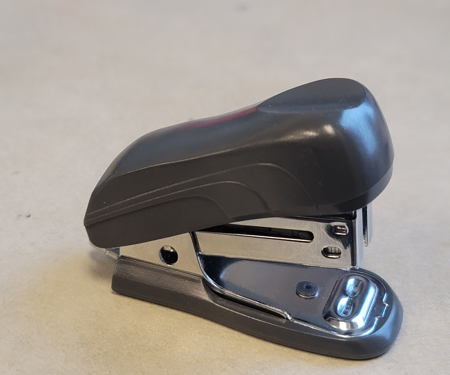
\includegraphics[width=0.45\textwidth]{../My_Code/Images/stapler_1.png}}
    \subcaptionbox{}{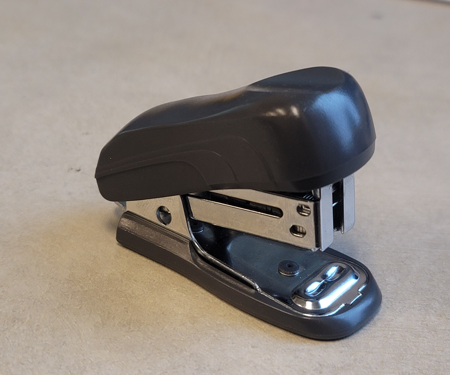
\includegraphics[width=0.45\textwidth]{../My_Code/Images/stapler_2.png}}
    \caption{Stereo image pairs (set 1)}
    \label{fig:stereo_im_1}
\end{figure}
\begin{figure}[!htbp]
     \centering
     \captionsetup[subfigure]{labelformat=empty}
    \subcaptionbox{}{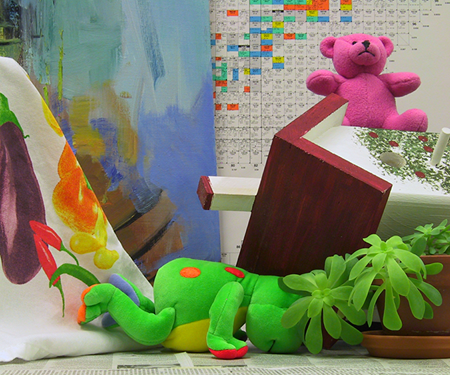
\includegraphics[width=0.45\textwidth]{../My_Code/Images/im2.png}}
    \subcaptionbox{}{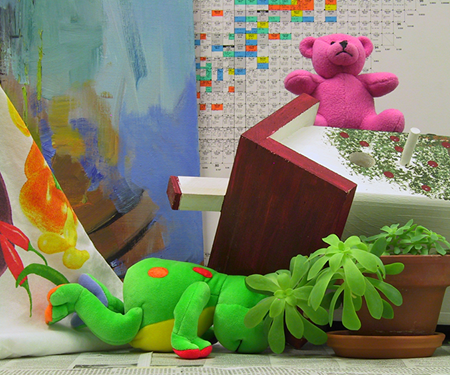
\includegraphics[width=0.45\textwidth]{../My_Code/Images/im6.png}}
    \caption{Stereo image pairs (set 2)}
    \label{fig:stereo_im_2}
\end{figure}

\newpage
\subsection{Manual Interest Point Selection}
\begin{figure}[!htbp]
     \centering
     \captionsetup[subfigure]{labelformat=empty}
    \subcaptionbox{}{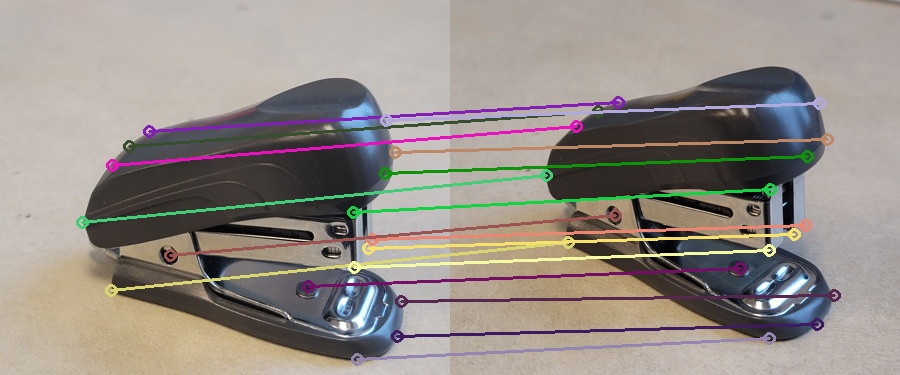
\includegraphics[width=0.90\textwidth]{../My_Code/Results/stapler_Original_Correspondences.jpg}}
    \caption{Manual correspondence of stereo image pair 1}
    \label{fig:orig_corr_1}
\end{figure}
\begin{figure}[!htbp]
     \centering
     \captionsetup[subfigure]{labelformat=empty}
    \subcaptionbox{}{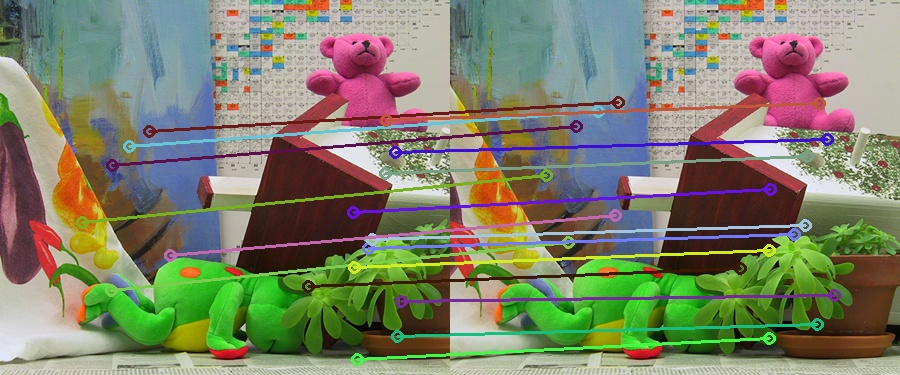
\includegraphics[width=0.90\textwidth]{../My_Code/Results/im2_Original_Correspondences.jpg}}
    \caption{Manual correspondence of stereo image pair 2}
    \label{fig:orig_corr_2}
\end{figure}

\newpage
\subsection{Epipolar Lines}
\begin{figure}[!htbp]
     \centering
     \captionsetup[subfigure]{labelformat=empty}
    \subcaptionbox{}{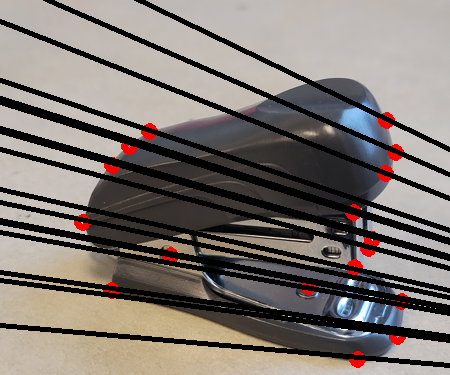
\includegraphics[width=0.45\textwidth]{../My_Code/Results/stapler_1_epilines.png}}
    \subcaptionbox{}{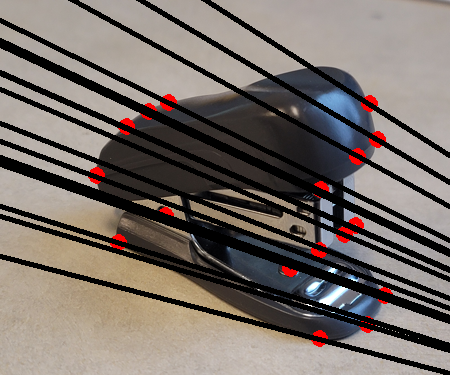
\includegraphics[width=0.45\textwidth]{../My_Code/Results/stapler_2_epilines.png}}
    \caption{Epipolar  lines of stereo image pair 1 before rectification}
    \label{fig:eipole_1}
\end{figure}
\begin{figure}[!htbp]
     \centering
     \captionsetup[subfigure]{labelformat=empty}
    \subcaptionbox{}{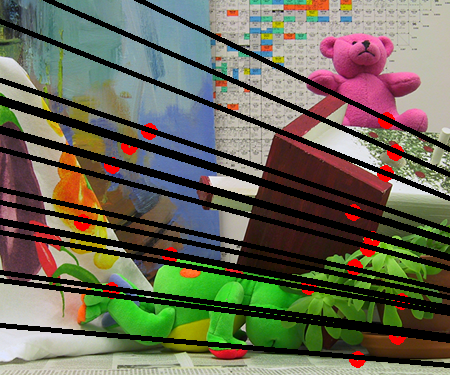
\includegraphics[width=0.45\textwidth]{../My_Code/Results/im2_epilines.png}}
    \subcaptionbox{}{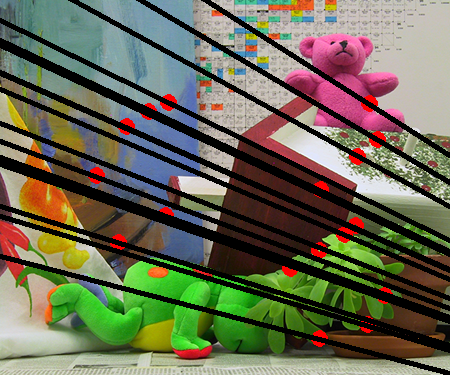
\includegraphics[width=0.45\textwidth]{../My_Code/Results/im6_epilines.png}}
    \caption{Epipolar  lines of stereo image pair 2 before rectification}
    \label{fig:eipole_2}
\end{figure}


\newpage
\subsection{Rectified Images}
\begin{figure}[!htbp]
     \centering
     \captionsetup[subfigure]{labelformat=empty}
    \subcaptionbox{}{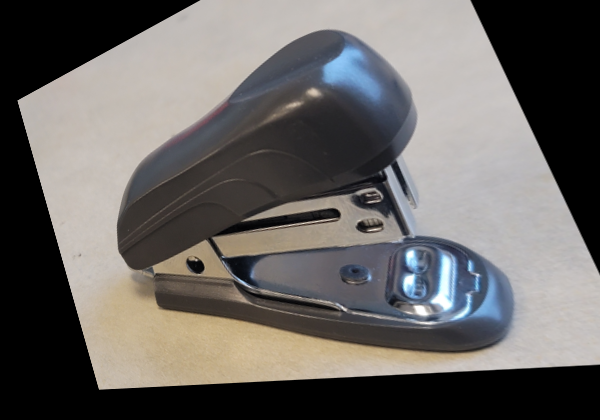
\includegraphics[width=0.45\textwidth]{../My_Code/Results/stapler_1_rectified.png}}
    \subcaptionbox{}{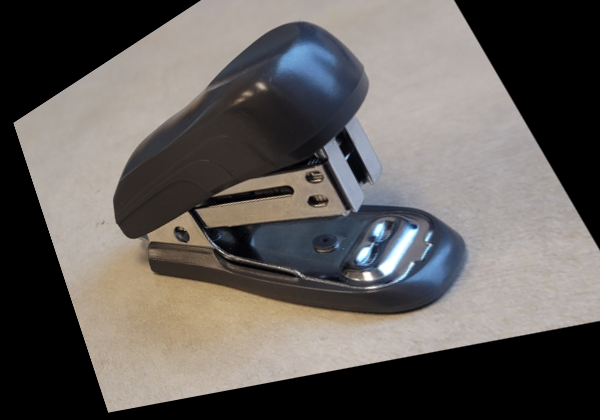
\includegraphics[width=0.45\textwidth]{../My_Code/Results/stapler_2_rectified.png}}
    \caption{Rectified images of stereo image pair 1}
    \label{fig:rect_1}
\end{figure}
\begin{figure}[!htbp]
     \centering
     \captionsetup[subfigure]{labelformat=empty}
    \subcaptionbox{}{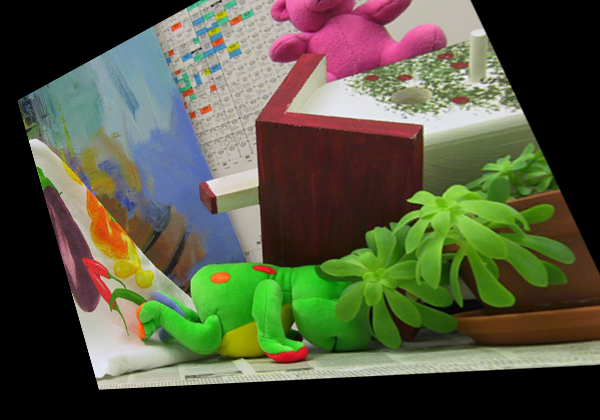
\includegraphics[width=0.45\textwidth]{../My_Code/Results/im2_rectified.png}}
    \subcaptionbox{}{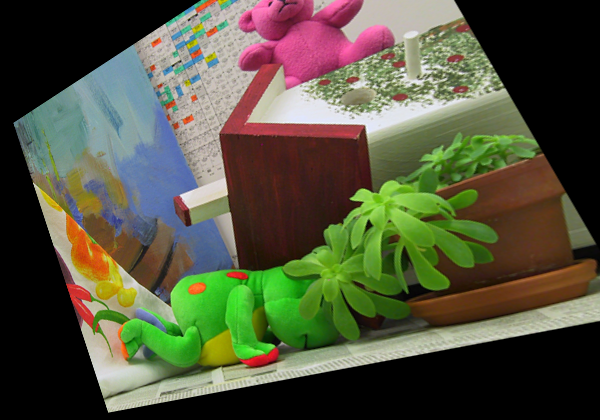
\includegraphics[width=0.45\textwidth]{../My_Code/Results/im6_rectified.png}}
    \caption{Rectified images of stereo image pair 2}
    \label{fig:rect_2}
\end{figure}



\newpage
\subsection{Rectified Correspondence for verification}
\begin{figure}[!htbp]
     \centering
     \captionsetup[subfigure]{labelformat=empty}
    \subcaptionbox{}{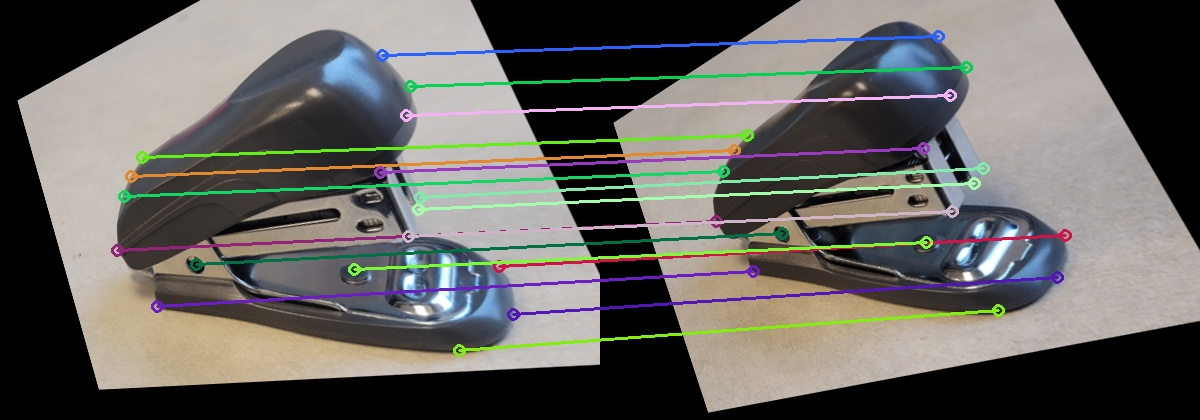
\includegraphics[width=0.90\textwidth]{../My_Code/Results/stapler_Rectified_Correspondences.jpg}}
    \caption{Rectified correspondences of stereo image pair 1}
    \label{fig:rect_corr_1}
\end{figure}
\begin{figure}[!htbp]
     \centering
     \captionsetup[subfigure]{labelformat=empty}
    \subcaptionbox{}{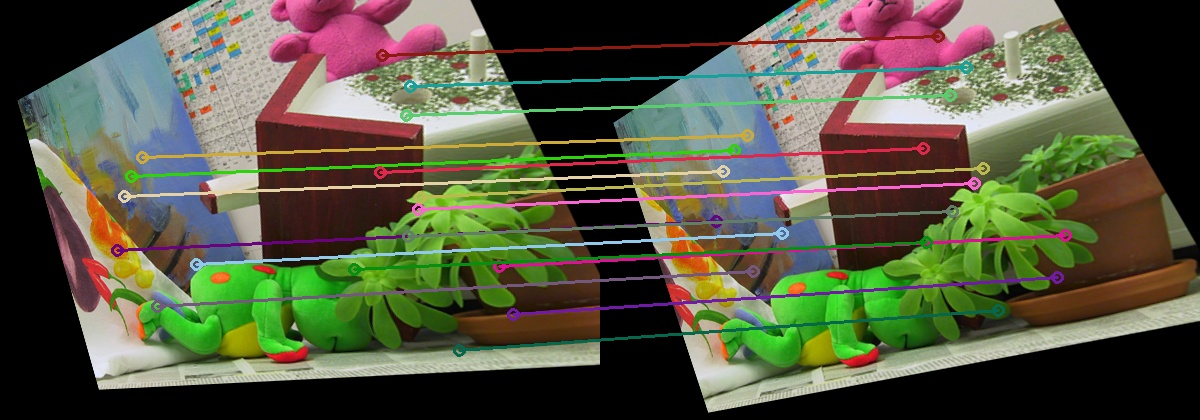
\includegraphics[width=0.90\textwidth]{../My_Code/Results/im2_Rectified_Correspondences.jpg}}
    \caption{Rectified correspondences of stereo image pair 2}
    \label{fig:rect_corr_2}
\end{figure}


\newpage
\subsection{Canny Edge Detection}
\begin{figure}[!htbp]
     \centering
     \captionsetup[subfigure]{labelformat=empty}
     \subcaptionbox{}{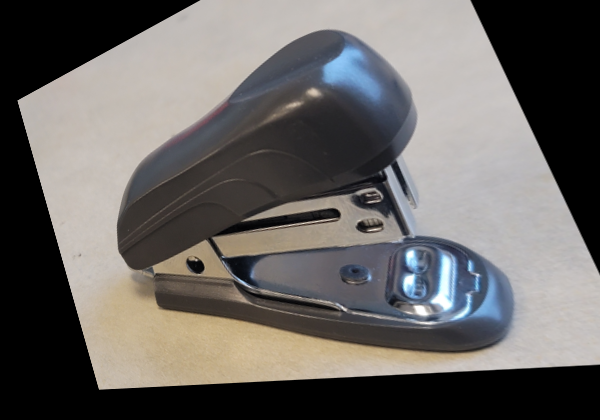
\includegraphics[width=0.30\textwidth]{../My_Code/Results/stapler_1_rectified.png}}
    \subcaptionbox{}{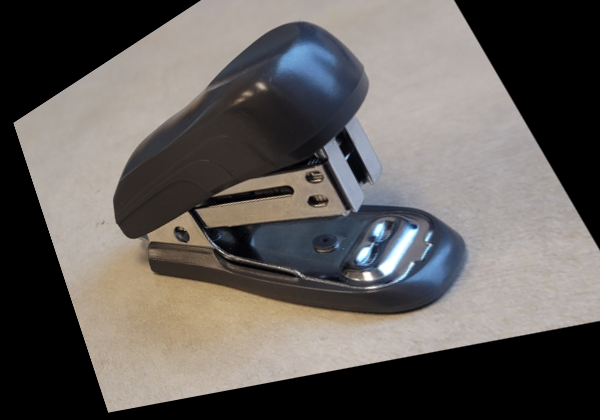
\includegraphics[width=0.30\textwidth]{../My_Code/Results/stapler_2_rectified.png}}\\
    \subcaptionbox{}{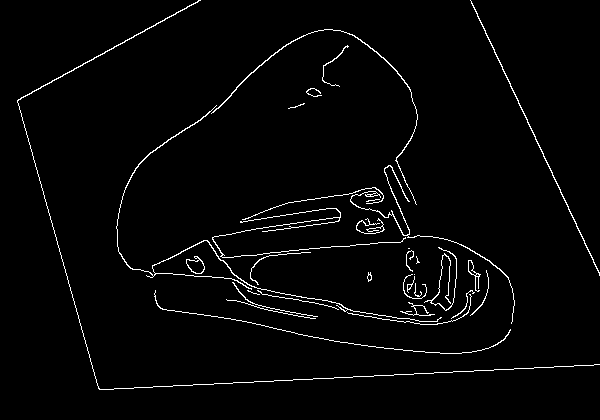
\includegraphics[width=0.30\textwidth]{../My_Code/Results/stapler_1_int_points_canny.png}}
    \subcaptionbox{}{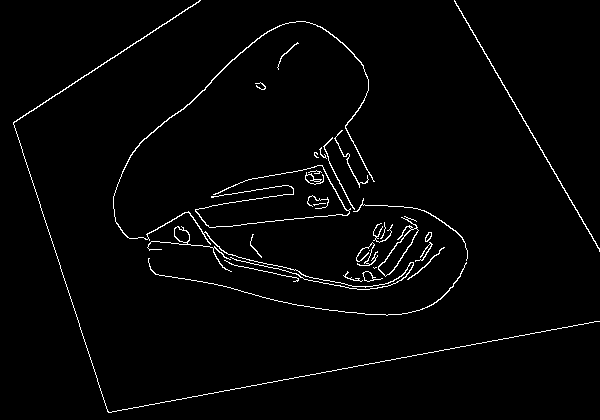
\includegraphics[width=0.30\textwidth]{../My_Code/Results/stapler_2_int_points_canny.png}}
    \caption{Canny edge map from OpenCV's implementation for stereo rectified image pair 1}
    \label{fig:canny_1}
\end{figure}
\begin{figure}[!htbp]
     \centering
     \captionsetup[subfigure]{labelformat=empty}
     \subcaptionbox{}{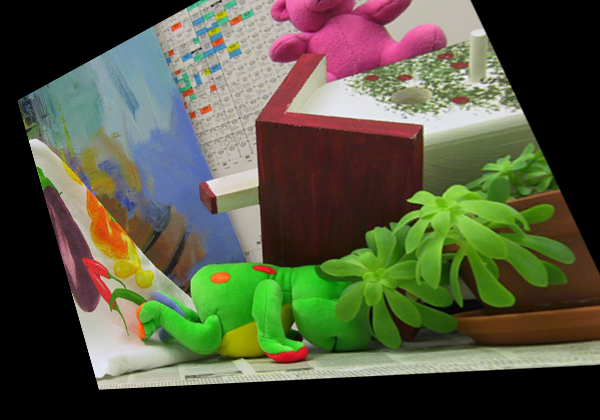
\includegraphics[width=0.30\textwidth]{../My_Code/Results/im2_rectified.png}}
    \subcaptionbox{}{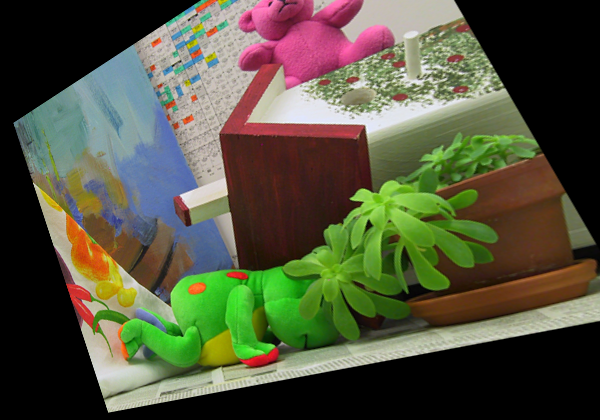
\includegraphics[width=0.30\textwidth]{../My_Code/Results/im6_rectified.png}}\\
    \subcaptionbox{}{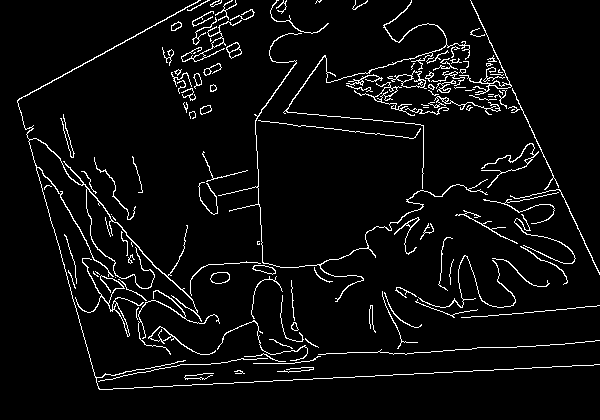
\includegraphics[width=0.30\textwidth]{../My_Code/Results/im2_int_points_canny.png}}
    \subcaptionbox{}{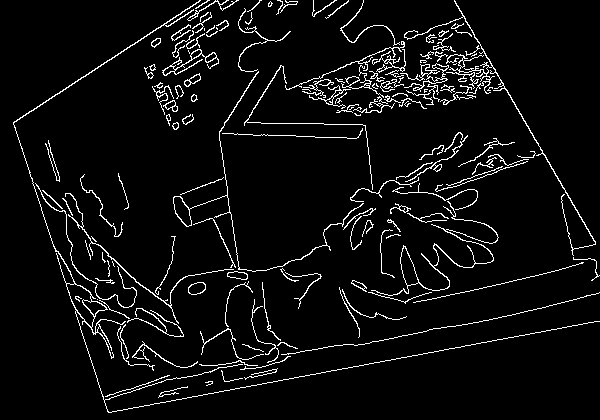
\includegraphics[width=0.30\textwidth]{../My_Code/Results/im6_int_points_canny.png}}
    \caption{Canny edge map from OpenCV's implementation for stereo rectified image pair 2}
    \label{fig:canny_2}
\end{figure}


\newpage
\subsection{Automatic Interest Point Detection}
\begin{figure}[!htbp]
     \centering
     \captionsetup[subfigure]{labelformat=empty}
    \subcaptionbox{}{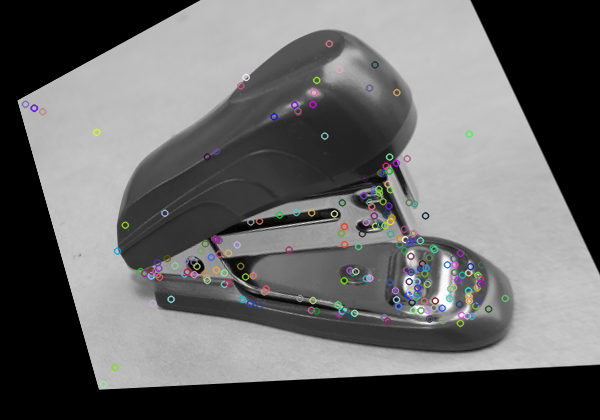
\includegraphics[width=0.30\textwidth]{../My_Code/Results/stapler_1_int_points_opencv.png}}
    \subcaptionbox{}{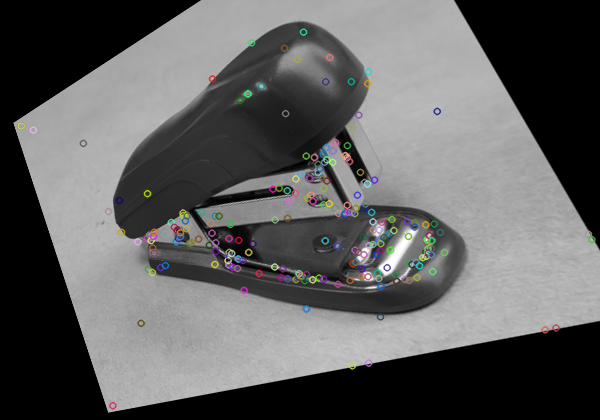
\includegraphics[width=0.30\textwidth]{../My_Code/Results/stapler_2_int_points_opencv.png}}
    \caption{Interest points from Canny edge map from OpenCV's implementation for stereo rectified image pair 1}
    \label{fig:canny_int_1}
\end{figure}
\begin{figure}[!htbp]
     \centering
     \captionsetup[subfigure]{labelformat=empty}
    \subcaptionbox{}{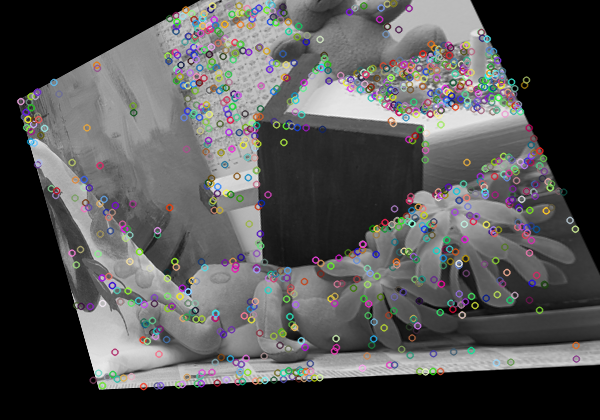
\includegraphics[width=0.28\textwidth]{../My_Code/Results/im2_int_points_opencv.png}}
    \subcaptionbox{}{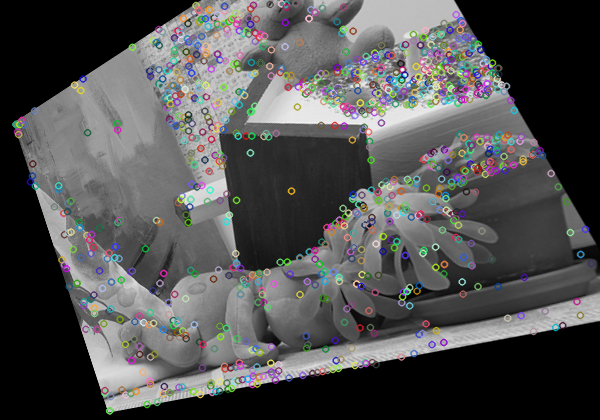
\includegraphics[width=0.28\textwidth]{../My_Code/Results/im6_int_points_opencv.png}}
    \caption{Interest points from Canny edge map from OpenCV's implementation for stereo rectified image pair 2}
    \label{fig:canny_int_2}
\end{figure}
\subsection{Automatic Correspondence Generation}
\begin{figure}[!htbp]
     \centering
     \captionsetup[subfigure]{labelformat=empty}
    \subcaptionbox{}{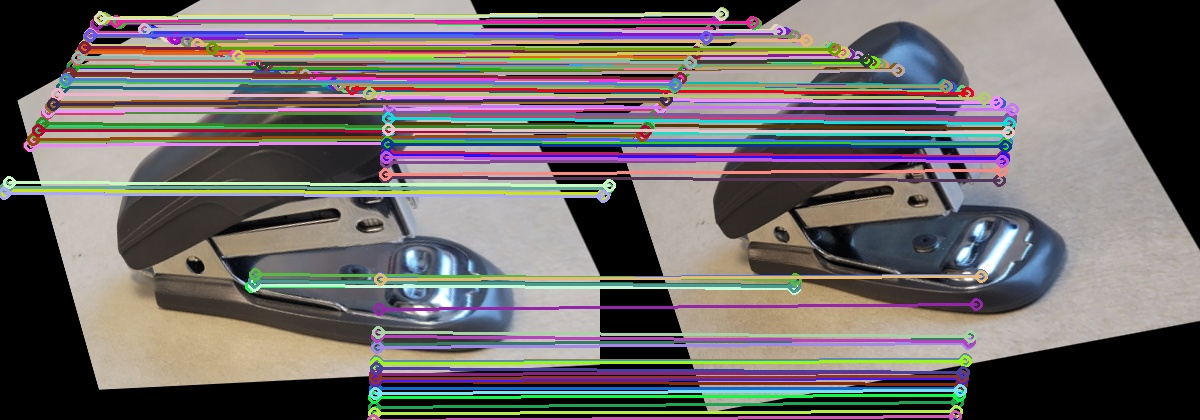
\includegraphics[width=0.55\textwidth]{../My_Code/Results/stapler_SSD_correspondence.jpg}}
    \caption{Rectified automatic correspondences of stereo pair 1 using SSD metric. Only a few correspondences are shown.}
    \label{fig:auto_rect_corr_1}
\end{figure}
\begin{figure}[!htbp]
     \centering
     \captionsetup[subfigure]{labelformat=empty}
    \subcaptionbox{}{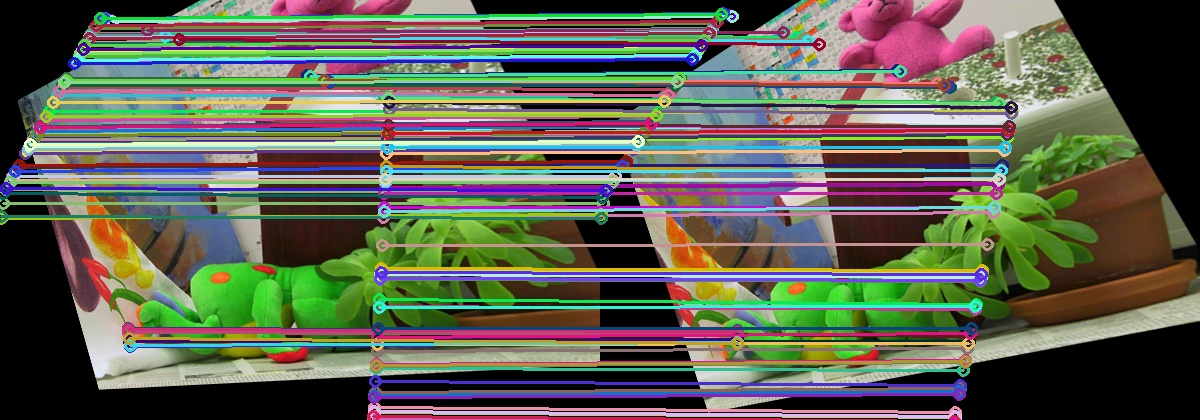
\includegraphics[width=0.55\textwidth]{../My_Code/Results/im2_SSD_correspondence.jpg}}
    \caption{Rectified automatic correspondences of stereo pair 2 using SSD metric. Only a few correspondences are shown.}
    \label{fig:auto_rect_corr_2}
\end{figure}


\newpage
\subsection{3D Visualization}
\begin{figure}[!htbp]
     \centering
     \captionsetup[subfigure]{labelformat=empty}
    \subcaptionbox{a}{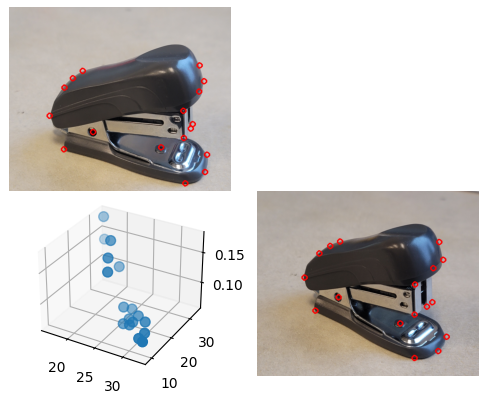
\includegraphics[width=0.495\textwidth]{../My_Code/Results/stapler_3D_plot_cropped.png}}
    \subcaptionbox{b}{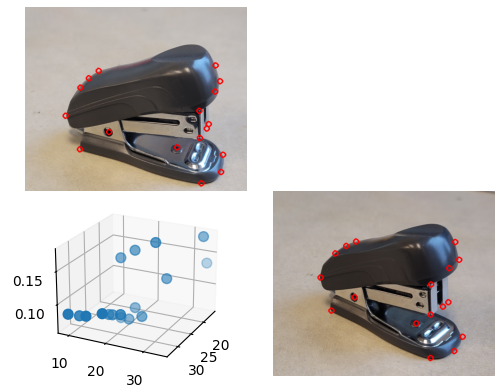
\includegraphics[width=0.495\textwidth]{../My_Code/Results/stapler_3D_plot_view_2_cropped.png}}
    \caption{3D view of the stereo projective resconstruction for image stereo pair 1 at two diffferent views.}
    \label{fig:3D_vis_1}
\end{figure}
\begin{figure}[!htbp]
     \centering
     \captionsetup[subfigure]{labelformat=empty}
    \subcaptionbox{a}{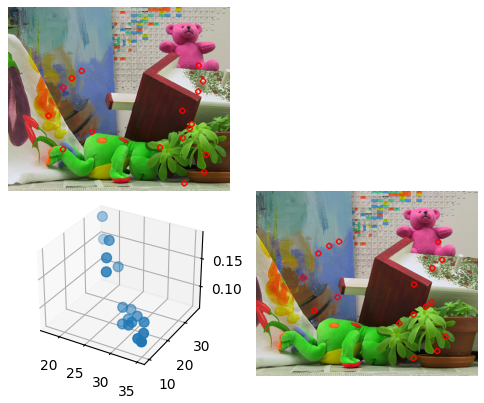
\includegraphics[width=0.495\textwidth]{../My_Code/Results/im2_3D_plot_cropped.png}}
    \subcaptionbox{b}{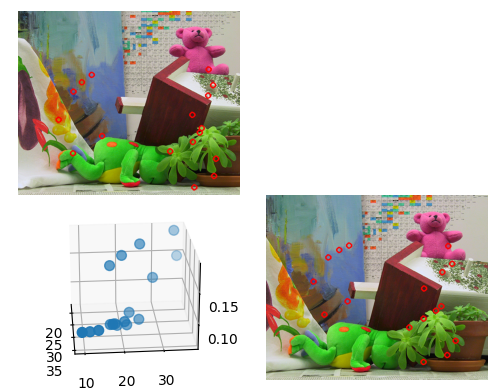
\includegraphics[width=0.495\textwidth]{../My_Code/Results/im2_3D_plot_view_2_cropped.png}}
    \caption{3D view of the stereo projective resconstruction for image stereo pair 2 at two diffferent views.}
    \label{fig:3D_vis_2}
\end{figure}


\newpage
\subsection{Loop and Zhang Algorithm Output}
\begin{figure}[!htbp]
     \centering
     \captionsetup[subfigure]{labelformat=empty}
    \subcaptionbox{a}{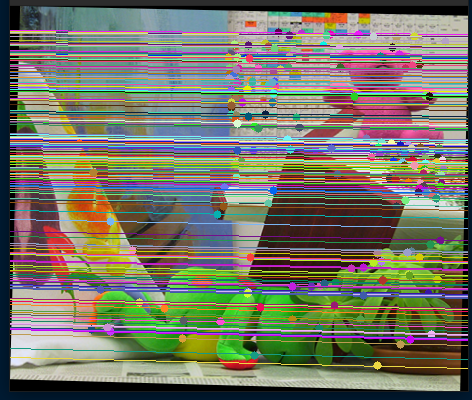
\includegraphics[width=0.495\textwidth]{../My_Code/Results/task_2_im2.png}}
    \subcaptionbox{b}{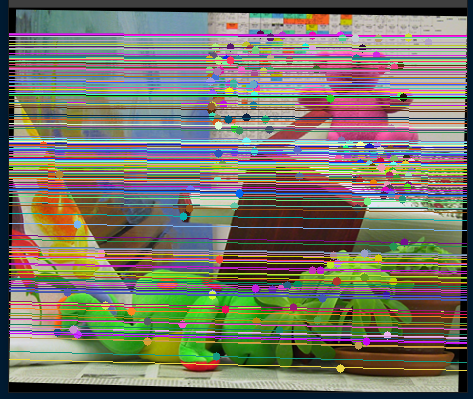
\includegraphics[width=0.495\textwidth]{../My_Code/Results/task_2_im6.png}}
    \caption{Image rectification from the loop and zhang algorithm for image stereo pair 2}
    \label{fig:lZ_2}
\end{figure}
\begin{figure}[!htbp]
     \centering
     \captionsetup[subfigure]{labelformat=empty}
    \subcaptionbox{a}{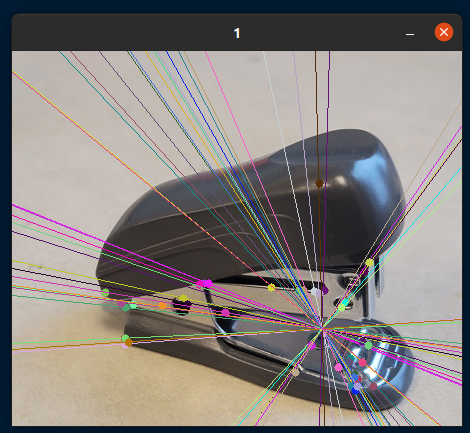
\includegraphics[width=0.495\textwidth]{../My_Code/Results/task_2_stapler_1_br.png}}
    \subcaptionbox{b}{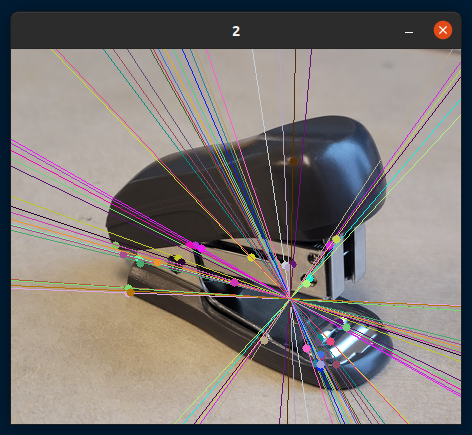
\includegraphics[width=0.495\textwidth]{../My_Code/Results/task_2_stapler_2_br.png}}
    \caption{Epipolar lines from the loop and zhang algorithm for image stereo pair 1 before rectification. It seems the algorithm can't approximate the epipolar lines for the chosen image stereo pair.}
    \label{fig:lZ_1}
\end{figure}


\subsection*{Comment}
It seems for the second pair of stereo images (Fig. \ref{fig:lZ_2}), the rectification from loop and Zhang algorithm and the custom implementation (Fig. \ref{fig:rect_corr_2}) are very similar. However, for the first pair of stereo images (Fig. \ref{fig:lZ_1}), the rectification is not so good as the custom implementation (Fig. \ref{fig:rect_corr_1}). It's not quite understandable at this stage of analysis, why the rectification is good for some pairs, but not for other pairs. It could be that, if the image pairs are taken from two widely different viewpoints (Camera angles with respect to the world coordinate point), the algorithm finds it difficult to estimate the homographies. 


\newpage
\subsection{Disparity Maps}
\begin{figure}[!htbp]
     \centering
     \captionsetup[subfigure]{labelformat=empty}
    \subcaptionbox{}{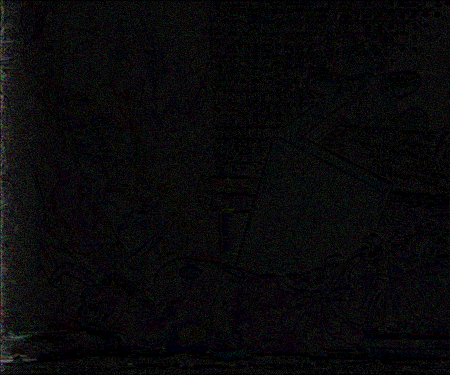
\includegraphics[width=0.245\textwidth]{../My_Code/Results/Disparity_Map_M_3_dmax_52.png}}
    \subcaptionbox{}{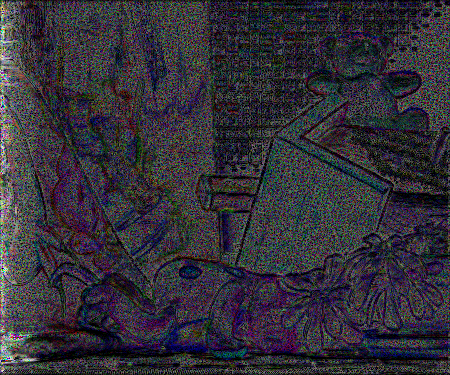
\includegraphics[width=0.245\textwidth]{../My_Code/Results/Disparity_Map_M_5_dmax_52.png}}
    \subcaptionbox{}{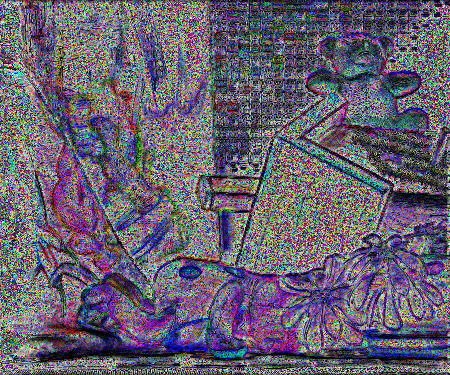
\includegraphics[width=0.245\textwidth]{../My_Code/Results/Disparity_Map_M_7_dmax_52.png}}
    \subcaptionbox{}{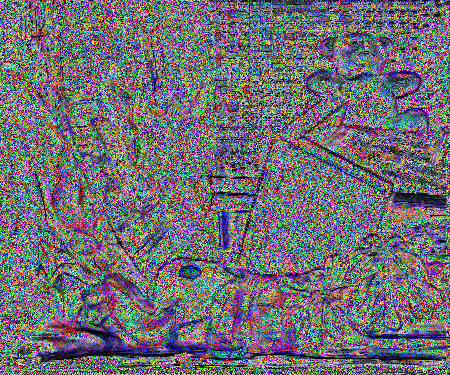
\includegraphics[width=0.245\textwidth]{../My_Code/Results/Disparity_Map_M_9_dmax_52.png}}
    \subcaptionbox{}{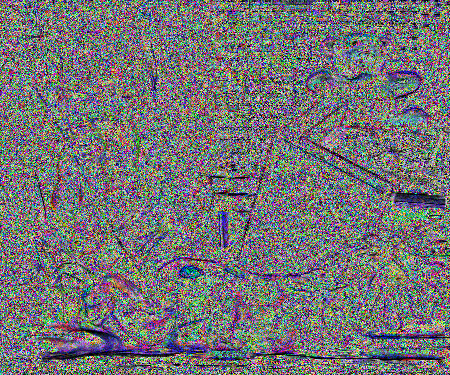
\includegraphics[width=0.245\textwidth]{../My_Code/Results/Disparity_Map_M_11_dmax_52.png}}
    \subcaptionbox{}{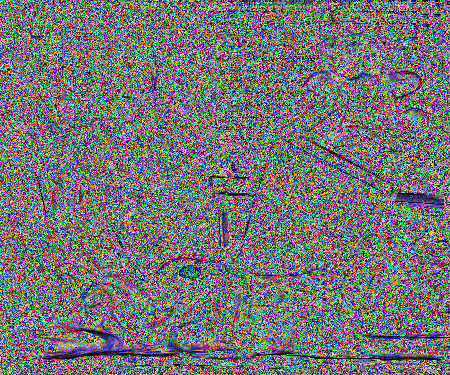
\includegraphics[width=0.245\textwidth]{../My_Code/Results/Disparity_Map_M_13_dmax_52.png}}
    \subcaptionbox{}{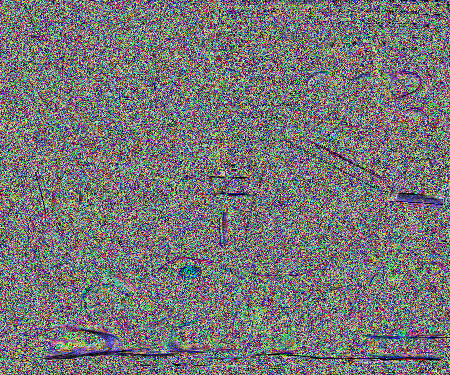
\includegraphics[width=0.245\textwidth]{../My_Code/Results/Disparity_Map_M_15_dmax_52.png}}
    \subcaptionbox{}{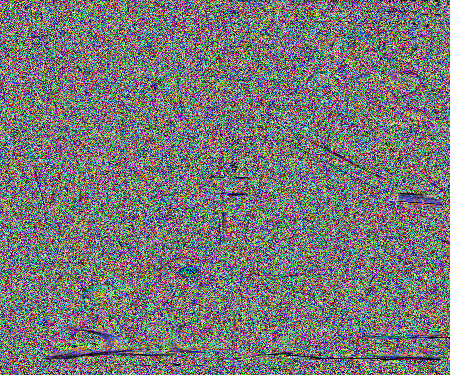
\includegraphics[width=0.245\textwidth]{../My_Code/Results/Disparity_Map_M_17_dmax_52.png}}
    \subcaptionbox{}{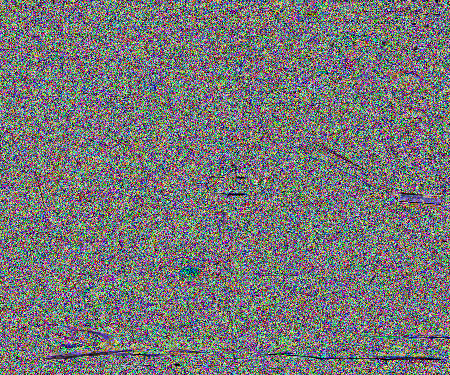
\includegraphics[width=0.245\textwidth]{../My_Code/Results/Disparity_Map_M_19_dmax_52.png}}
    \subcaptionbox{}{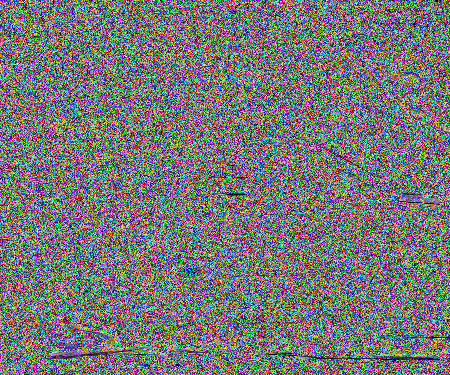
\includegraphics[width=0.245\textwidth]{../My_Code/Results/Disparity_Map_M_21_dmax_52.png}}
    \subcaptionbox{}{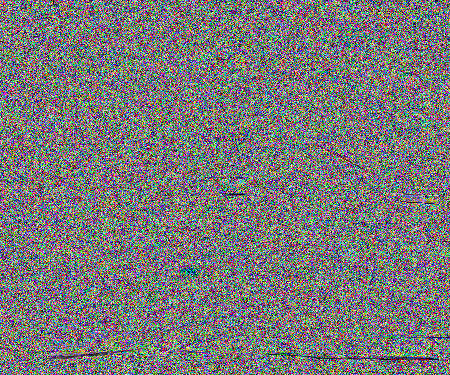
\includegraphics[width=0.245\textwidth]{../My_Code/Results/Disparity_Map_M_23_dmax_52.png}}
    \subcaptionbox{}{
\includegraphics[width=0.245\textwidth]{../My_Code/Results/Disparity_Map_M_25_dmax_52.png}}
    \subcaptionbox{}{\includegraphics[width=0.245\textwidth]{../My_Code/Results/Disparity_Map_M_27_dmax_52.png}}
    \subcaptionbox{}{\includegraphics[width=0.245\textwidth]{../My_Code/Results/Disparity_Map_M_29_dmax_52.png}}
    \subcaptionbox{}{\includegraphics[width=0.245\textwidth]{../My_Code/Results/Disparity_Map_M_31_dmax_52.png}}
    \subcaptionbox{}{\includegraphics[width=0.245\textwidth]{../My_Code/Results/Disparity_Map_M_33_dmax_52.png}}
    \subcaptionbox{}{\includegraphics[width=0.245\textwidth]{../My_Code/Results/Disparity_Map_M_35_dmax_52.png}}
    \subcaptionbox{}{\includegraphics[width=0.245\textwidth]{../My_Code/Results/Disparity_Map_M_37_dmax_52.png}}
    \caption{Disparity maps for stereo image pairs. From (top to bottom, in raster order scanning, M=3,5,7,...,37. The disparity maps are calculuted separately for three different channels and the maps are plotted in RGB format. Here, delta = 2}
    \label{fig:disparity}
\end{figure}


\newpage
\subsection{Disparity Error Maps}
\begin{figure}[!htbp]
     \centering
     \captionsetup[subfigure]{labelformat=empty}
    \subcaptionbox{}{\includegraphics[width=0.245\textwidth]{../My_Code/Results/Disparity_Map_Error_M_3_dmax_52.png}}
    \subcaptionbox{}{\includegraphics[width=0.245\textwidth]{../My_Code/Results/Disparity_Map_Error_M_5_dmax_52.png}}
    \subcaptionbox{}{\includegraphics[width=0.245\textwidth]{../My_Code/Results/Disparity_Map_Error_M_7_dmax_52.png}}
    \subcaptionbox{}{\includegraphics[width=0.245\textwidth]{../My_Code/Results/Disparity_Map_Error_M_9_dmax_52.png}}
    \subcaptionbox{}{\includegraphics[width=0.245\textwidth]{../My_Code/Results/Disparity_Map_Error_M_11_dmax_52.png}}
    \subcaptionbox{}{\includegraphics[width=0.245\textwidth]{../My_Code/Results/Disparity_Map_Error_M_13_dmax_52.png}}
    \subcaptionbox{}{\includegraphics[width=0.245\textwidth]{../My_Code/Results/Disparity_Map_Error_M_15_dmax_52.png}}
    \subcaptionbox{}{\includegraphics[width=0.245\textwidth]{../My_Code/Results/Disparity_Map_Error_M_17_dmax_52.png}}
    \subcaptionbox{}{\includegraphics[width=0.245\textwidth]{../My_Code/Results/Disparity_Map_Error_M_19_dmax_52.png}}
    \subcaptionbox{}{\includegraphics[width=0.245\textwidth]{../My_Code/Results/Disparity_Map_Error_M_21_dmax_52.png}}
    \subcaptionbox{}{\includegraphics[width=0.245\textwidth]{../My_Code/Results/Disparity_Map_Error_M_23_dmax_52.png}}
    \subcaptionbox{}{\includegraphics[width=0.245\textwidth]{../My_Code/Results/Disparity_Map_Error_M_25_dmax_52.png}}
    \subcaptionbox{}{\includegraphics[width=0.245\textwidth]{../My_Code/Results/Disparity_Map_Error_M_27_dmax_52.png}}
    \subcaptionbox{}{\includegraphics[width=0.245\textwidth]{../My_Code/Results/Disparity_Map_Error_M_29_dmax_52.png}}
    \subcaptionbox{}{\includegraphics[width=0.245\textwidth]{../My_Code/Results/Disparity_Map_Error_M_31_dmax_52.png}}
    \subcaptionbox{}{\includegraphics[width=0.245\textwidth]{../My_Code/Results/Disparity_Map_Error_M_33_dmax_52.png}}
    \subcaptionbox{}{\includegraphics[width=0.245\textwidth]{../My_Code/Results/Disparity_Map_Error_M_35_dmax_52.png}}
    \subcaptionbox{}{\includegraphics[width=0.245\textwidth]{../My_Code/Results/Disparity_Map_Error_M_37_dmax_52.png}}
    \caption{Disparity error maps for stereo image pairs. From (top to bottom, in raster order scanning, M=3,5,7,...,37. The disparity maps are calculuted separately for three different channels and the maps are plotted in RGB format. Here, delta = 2}
    \label{fig:disp_error}
\end{figure}



\newpage
\subsection{Disparity Error Masks}
\begin{figure}[!htbp]
     \centering
     \captionsetup[subfigure]{labelformat=empty}
    \subcaptionbox{}{\includegraphics[width=0.245\textwidth]{../My_Code/Results/Disparity_Map_Error_Mask_M_3_dmax_52.png}}
    \subcaptionbox{}{\includegraphics[width=0.245\textwidth]{../My_Code/Results/Disparity_Map_Error_Mask_M_5_dmax_52.png}}
    \subcaptionbox{}{\includegraphics[width=0.245\textwidth]{../My_Code/Results/Disparity_Map_Error_Mask_M_7_dmax_52.png}}
    \subcaptionbox{}{\includegraphics[width=0.245\textwidth]{../My_Code/Results/Disparity_Map_Error_Mask_M_9_dmax_52.png}}
    \subcaptionbox{}{\includegraphics[width=0.245\textwidth]{../My_Code/Results/Disparity_Map_Error_Mask_M_11_dmax_52.png}}
    \subcaptionbox{}{\includegraphics[width=0.245\textwidth]{../My_Code/Results/Disparity_Map_Error_Mask_M_13_dmax_52.png}}
    \subcaptionbox{}{\includegraphics[width=0.245\textwidth]{../My_Code/Results/Disparity_Map_Error_Mask_M_15_dmax_52.png}}
    \subcaptionbox{}{\includegraphics[width=0.245\textwidth]{../My_Code/Results/Disparity_Map_Error_Mask_M_17_dmax_52.png}}
    \subcaptionbox{}{\includegraphics[width=0.245\textwidth]{../My_Code/Results/Disparity_Map_Error_Mask_M_19_dmax_52.png}}
    \subcaptionbox{}{\includegraphics[width=0.245\textwidth]{../My_Code/Results/Disparity_Map_Error_Mask_M_21_dmax_52.png}}
    \subcaptionbox{}{\includegraphics[width=0.245\textwidth]{../My_Code/Results/Disparity_Map_Error_Mask_M_23_dmax_52.png}}
    \subcaptionbox{}{\includegraphics[width=0.245\textwidth]{../My_Code/Results/Disparity_Map_Error_Mask_M_25_dmax_52.png}}
    \subcaptionbox{}{\includegraphics[width=0.245\textwidth]{../My_Code/Results/Disparity_Map_Error_Mask_M_27_dmax_52.png}}
    \subcaptionbox{}{\includegraphics[width=0.245\textwidth]{../My_Code/Results/Disparity_Map_Error_Mask_M_29_dmax_52.png}}
    \subcaptionbox{}{\includegraphics[width=0.245\textwidth]{../My_Code/Results/Disparity_Map_Error_Mask_M_31_dmax_52.png}}
    \subcaptionbox{}{\includegraphics[width=0.245\textwidth]{../My_Code/Results/Disparity_Map_Error_Mask_M_33_dmax_52.png}}
    \subcaptionbox{}{\includegraphics[width=0.245\textwidth]{../My_Code/Results/Disparity_Map_Error_Mask_M_35_dmax_52.png}}
    \subcaptionbox{}{\includegraphics[width=0.245\textwidth]{../My_Code/Results/Disparity_Map_Error_Mask_M_37_dmax_52.png}}
    \caption{Disparity error masks for stereo image pairs. From (top to bottom, in raster order scanning, M=3,5,7,...,37. The disparity maps are calculuted separately for three different channels and the maps are plotted in RGB format. Here, delta = 2}
    \label{fig:disp_mask}
\end{figure}


\newpage
\subsection{Disparity Accuracy}
\begin{figure}[!htbp]
     \centering
     \captionsetup[subfigure]{labelformat=empty}
    \subcaptionbox{a}{\includegraphics[width=0.65\textwidth]{../My_Code/Results/Disparity_Accuracy.png}}
    \caption{Disparity accuracy. It seems the accuracy peaks near M=9 or 10. However, as delta increases, the peak accuracy increases. hence, it's almost ensured, the two disparity maps (ground truth and estimated) are need to be normalized.}
    \label{fig:disp_acc}
\end{figure}
\subsection*{Comments}
The disparity map becomes optimal with peak accuracy and minimal error near M=9 or 10. To get the exact accuracy, the ground truth disparity maps and estimated disparity maps need to be normalized and saved using the same scaling factor.



\newpage
\section{References}
\begin{itemize}
\item[1] Richard Hartley and Andrew Zisserman. Multiple view geometry in computer vision. Cambridge university press, 2003.
\item[2] Daniel Scharstein and Richard Szeliski. A taxonomy and evaluation of
dense two-frame stereo correspondence algorithms. International journal
of computer vision, 47(1):7–42, 2002.
\item[3] Daniel Scharstein, Heiko Hirschmüller, York Kitajima, Greg Krathwohl,
Nera Nešić, Xi Wang, and Porter Westling. High-resolution stereo
datasets with subpixel-accurate ground truth. In German conference
on pattern recognition, pages 31–42. Springer, 2014.
\end{itemize}

\newpage
\section{Source Code - Task 1}
\begin{lstlisting}[language=Python]
import cv2
import os
import numpy as np
import random
import matplotlib.pyplot as plt
from matplotlib.patches import ConnectionPatch
from scipy import optimize

def opencv_interest_points(img,name):
	gray= cv2.cvtColor(img,cv2.COLOR_BGR2GRAY)
	sift = cv2.SIFT_create()
	kp,des = sift.detectAndCompute(gray,None)
	img=cv2.drawKeypoints(gray,kp,img)
	cv2.imwrite(name,img)
	return img,kp,des
def opencv_correspondence(img_1,kp_1,des_1,img_2,kp_2,des_2,name,N):
	#N 	: how many correspondences to be kept
	bf = cv2.BFMatcher(cv2.NORM_L1, crossCheck=True)# create BFMatcher object
	matches = bf.match(des_1,des_2)# Match descriptors.
	matches = sorted(matches, key = lambda x:x.distance)# Sort them in the order of their distance.
	img3 = cv2.drawMatches(img_1,kp_1,img_2,kp_2,matches[:N], None,flags=2)# Draw first 10 matches.
	cv2.imwrite(name+'opencv_correspondences.jpg',img3)
def Sum_of_Squared_Differences(Im_1,Im_2,corner_indexes_1,corner_indexes_2,N,padding_mode='constant'):
	#N	: N*N neighbourhood
	I_1 = np.pad(Im_1,((int(N/2),int(N/2)),(int(N/2),int(N/2)),(0,0)),mode=padding_mode)
	I_2 = np.pad(Im_2,((int(N/2),int(N/2)),(int(N/2),int(N/2)),(0,0)),mode=padding_mode)
	Best_Matches = np.zeros((corner_indexes_1.shape[0],1))
	SSD_list = np.zeros((corner_indexes_1.shape[0],1))
	for s1 in range(0,corner_indexes_1.shape[0]):
		SSD = list()
		i = corner_indexes_1[s1,0]
		j = corner_indexes_1[s1,1]
		ix = i+int(N/2)
		jx = j+int(N/2)
		f_1 = I_1[ix-int(N/2):ix+int(N/2),jx-int(N/2):jx+int(N/2),0]
		for s2 in range(0,corner_indexes_2.shape[0]):
			i = corner_indexes_2[s2,0]
			j = corner_indexes_2[s2,1]
			ix = i+int(N/2)
			jx = j+int(N/2)
			f_2 = I_2[ix-int(N/2):ix+int(N/2),jx-int(N/2):jx+int(N/2),0]
			#if np.sum(f_2) !=0:
			SSD.append(np.sum(np.square(f_1.flatten() - f_2.flatten())))
		SSD = np.array(SSD).squeeze()
		ind = np.argsort(SSD)[0]
		Best_Matches[s1,0] = ind
		SSD_list[s1,0] = SSD[ind]
	return Best_Matches,SSD_list
def Normalized_Cross_Correlations(Im_1,Im_2,corner_indexes_1,corner_indexes_2,N,padding_mode='constant'):
	#N	: N*N neighbourhood
	I_1 = np.pad(Im_1,((int(N/2),int(N/2)),(int(N/2),int(N/2)),(0,0)),mode=padding_mode)
	I_2 = np.pad(Im_2,((int(N/2),int(N/2)),(int(N/2),int(N/2)),(0,0)),mode=padding_mode)
	Best_Matches = np.zeros((corner_indexes_1.shape[0],1))
	NCC_list = np.zeros((corner_indexes_1.shape[0],1))
	for s1 in range(0,corner_indexes_1.shape[0]):
		i = corner_indexes_1[s1,0]
		j = corner_indexes_1[s1,1]
		ix = i+int(N/2)
		jx = j+int(N/2)
		f_1 = I_1[ix-int(N/2):ix+int(N/2),jx-int(N/2):jx+int(N/2),0]
		m_1 = np.mean(I_1[ix-int(N/2):ix+int(N/2),jx-int(N/2):jx+int(N/2),0])
		NCC = np.zeros((corner_indexes_2.shape[0],1))
		for s2 in range(0,corner_indexes_2.shape[0]):
			i = corner_indexes_2[s2,0]
			j = corner_indexes_2[s2,1]
			ix = i+int(N/2)
			jx = j+int(N/2)
			f_2 = I_2[ix-int(N/2):ix+int(N/2),jx-int(N/2):jx+int(N/2),0]
			m_2 = np.mean(I_2[ix-int(N/2):ix+int(N/2),jx-int(N/2):jx+int(N/2),0])
			num = np.sum(np.multiply((f_1-m_1),(f_2-m_2)))
			den = np.sqrt(np.multiply(np.sum(np.square(f_1-m_1)),np.sum(np.square(f_2-m_2))))
			if den != 0:
				NCC[s2,0] = num/den
		NCC = NCC.squeeze()
		ind = np.argsort(NCC)[0]
		Best_Matches[s1,0] = ind
		NCC_list[s1,0] = NCC[ind]
	return Best_Matches,NCC_list
def plot_correspondences(I_1,I_2,correspondences,M,name):
	#M	: how many correspondences to show
	CI = np.concatenate((I_1,I_2),axis=1)
	im_width = I_1.shape[1]
	if M<len(correspondences):
		ind = random.sample(np.arange(0,len(correspondences)).tolist(),M)
	else:
		ind = np.arange(0,len(correspondences))
	for ix in ind:
		color_matrix = (random.sample(np.arange(0,255).tolist(),1)[0],random.sample(np.arange(0,255).tolist(),1)[0],random.sample(np.arange(0,255).tolist(),1)[0])
		points_1 = tuple(correspondences[ix][0])
		points_2 = tuple([correspondences[ix][1][0]+im_width,correspondences[ix][1][1]])
		cv2.circle(CI,points_1,5,color_matrix,2)
		cv2.circle(CI,points_2,5,color_matrix,2)
		cv2.line(CI,points_1,points_2,color_matrix,2)
	cv2.imwrite('./Results/'+name+'.jpg',CI)
def physical_to_homogeneous(points):
	#points = n*2
	HC = np.concatenate((points,np.ones((points.shape[0],1))),axis=1)
	return HC.T
def homogeneous_to_physical(points):
	#points = 3*n
	physical_points = points[:,:]/points[-1,:]
	return physical_points[:-1,:].T
def data_normalization(points):
	#points = n*2
	mean_coord = np.mean(points,axis=0)
	distances = np.linalg.norm(points-mean_coord,axis=1)
	mean_distance = np.mean(distances)
	normalizing_factor = np.sqrt(2)/mean_distance
	T = np.zeros((3,3))
	T[0,0] = normalizing_factor
	T[0,2] = -normalizing_factor*mean_coord[0]
	T[1,1] = normalizing_factor
	T[1,2] = -normalizing_factor*mean_coord[1]
	T[2,2] = 1
	HC = physical_to_homogeneous(points)
	HC_normalized = np.matmul(T,HC)
	normalized_points = homogeneous_to_physical(HC_normalized)
	return normalized_points, T
def condition_F(F):
	U,D,V = np.linalg.svd(F)
	print(D)
	D[np.argmin(D)] = 0
	print(D)
	F_conditioned = np.matmul(U,np.matmul(np.diag(D),V))
	#F_conditioned = F_conditioned/F_conditioned[2,2]
	return F_conditioned
def Fundamental_Matrix(point_set_1,point_set_2,T1,T2):
	#estimate the fundamental matrix from interest point pairs
	#point_set_1 = shape:[N,2]
	#point_set_2 = shape:[N,2]
	#T1 = normalizing matrix for point_set_1
	#T2 = normalizing matrix for point_set_2
	A = np.zeros((point_set_1.shape[0],9))
	b = np.zeros((point_set_1.shape[0],1))
	for ix in range(0,point_set_1.shape[0]):
		A[ix,:] = [point_set_2[ix,0]*point_set_1[ix,0], point_set_2[ix,0]*point_set_1[ix,1], point_set_2[ix,0], point_set_2[ix,1]*point_set_1[ix,0], point_set_2[ix,1]*point_set_1[ix,1], point_set_2[ix,1], point_set_1[ix,0], point_set_1[ix,1], 1]
	U,D,V = np.linalg.svd(np.matmul(A.T,A))
	F = V[-1,:]
	F = np.reshape(F,[3,3])
	F = F/F[-1,-1]
	F = condition_F(F)
	F = np.matmul(T2.T,np.matmul(F,T1))
	F = F/F[-1,-1]
	return F
def calculate_epipoles(F):
	U,D,V = np.linalg.svd(F)
	left_epipole = V[-1,:].T
	right_epipole = U[:,-1]
	left_epipole = np.reshape(left_epipole/left_epipole[-1],[3,-1])
	right_epipole = np.reshape(right_epipole/right_epipole[-1],[3,-1])
	return left_epipole,right_epipole
def vector_to_matrix(X):
	X = X.squeeze()
	return np.array([[0,-X[2],X[1]],[X[2],0,-X[0]],[-X[1],X[0],0]])
def estimate_projection_matrices(F,left_epipole,right_epipole):
	P_left = np.concatenate((np.eye(3,dtype=float),np.zeros((3,1))),axis=1)
	temp = np.matmul(vector_to_matrix(right_epipole),F)
	P_right = np.concatenate((temp,right_epipole),axis=1)
	return P_left,P_right
def triangulate_points(point_set_1,point_set_2,P_left,P_right):
	triangulated_points = np.zeros((4,point_set_1.shape[0]))
	for ix in range(0,point_set_1.shape[0]):
		A=np.zeros((4,4))
		A[0,:] = point_set_1[ix,0]*P_left[2,:] - P_left[0,:]
		A[1,:] = point_set_1[ix,1]*P_left[2,:] - P_left[1,:]
		A[2,:] = point_set_2[ix,0]*P_right[2,:] - P_right[0,:]
		A[3,:] = point_set_2[ix,1]*P_right[2,:] - P_right[1,:]
		U,D,V = np.linalg.svd(np.matmul(A.T,A))
		X = V[-1,:]
		X = X/X[-1]
		triangulated_points[:,ix] = X.T
	return triangulated_points
def cost_function(P_right,point_set_1,point_set_2,P_left,triangulated_points):
	P_right = np.reshape(P_right,[3,4])
	reprojected_point_set_1 = np.matmul(P_left,triangulated_points)
	reprojected_point_set_2 = np.matmul(P_right,triangulated_points)
	reprojected_point_set_1 = reprojected_point_set_1[:-1,:]/reprojected_point_set_1[-1,:]
	reprojected_point_set_2 = reprojected_point_set_2[:-1,:]/reprojected_point_set_2[-1,:]
	error_1 = point_set_1-reprojected_point_set_1.T
	error_2 = point_set_2-reprojected_point_set_2.T
	error = np.square(error_1.flatten()) + np.square(error_2.flatten())
	return error
def nonlinear_optimization(point_set_1,point_set_2,P_left,P_right):
	triangulated_points = triangulate_points(point_set_1,point_set_2,P_left,P_right)
	parameters = P_right.flatten()
	lm_refined_P_right = optimize.least_squares(cost_function,parameters,args=[point_set_1,point_set_2,P_left,triangulated_points],method='lm',verbose=1,ftol=1e-15)
	lm_refined_P_right = np.reshape(lm_refined_P_right.x,[3,4])
	lm_refined_P_right = lm_refined_P_right / lm_refined_P_right[-1,-1]
	return P_left,lm_refined_P_right
def fundamental_matrix_from_projection(P_left,P_right):
	right_epipole = P_right[:,-1]
	right_epipole_x = vector_to_matrix(right_epipole)
	P_pseudo = np.matmul(P_left.T, np.linalg.inv(np.matmul(P_left,P_left.T)))
	F = np.matmul(right_epipole_x, np.matmul(P_right,P_pseudo))
	F = F/F[-1,-1]
	return F
def estimate_right_homography(image_2, image_2_pt_normalized, right_epipole_refined, P_right_refined):
	height, width = image_2.shape[0], image_2.shape[1]
	#Translation matrix to translate the image to the center
	T1 = np.array([[1., 0., -width/2.],[0., 1., -height/2.],[0., 0., 1.]])
	#Rotation matrix to rotate the epipolar line to x-axis
	phi = np.arctan((right_epipole_refined[1,0]-height/2.0)/(right_epipole_refined[0,0]-width/2.0))
	phi = -phi
	R = np.array([[np.cos(phi), -np.sin(phi), 0.],[np.sin(phi), np.cos(phi), 0.],[0.,0.,1.]])
	#compute the homography that translates epipole to infinity
	#f = np.linalg.norm(np.array([right_epipole_refined[1,0]-height/2.0, right_epipole_refined[0,0]-width/2.0]))
	f = np.cos(phi)*(right_epipole_refined[0,0]-width/2.0) - np.sin(phi)*(right_epipole_refined[1,0]-height/2.0)
	G = np.eye(3,dtype=float)
	G[2,0] = -1/f
	H_right = np.matmul(G,np.matmul(R,T1))
	#Translate the image back to original location
	img_2_center = transform_image(H_right,np.array([width/2.0,height/2.0]).reshape([1,2]))
	T2 = np.array([[1., 0., width/2.0-img_2_center[0,0]],[0., 1., height/2.0-img_2_center[0,1]],[0., 0., 1.]])
	H_right = np.matmul(T2,H_right)
	H_right = H_right/H_right[-1,-1]
	return H_right
def transform_image(H,input_data):
	input_data = input_data.T
	input_data = np.concatenate((input_data,np.ones((1,input_data.shape[1]))),axis=0)
	transformed_image = np.matmul(H,input_data)
	transformed_image = transformed_image[0:2,:]/transformed_image[2,:]
	return transformed_image[0:2,:].T
def estimate_left_homography(image_1,image_1_pt_normalized, image_2_pt_normalized, left_epipole_refined, P_left_refined, P_right_refined, H_right):
	height, width = image_1.shape[0], image_1.shape[1]
	T1 = np.array([[1., 0., -width/2.],[0., 1., -height/2.],[0., 0., 1.]])
	#Rotation matrix to rotate the epipolar line to x-axis
	phi = np.arctan((left_epipole_refined[1,0]-height/2.0)/(left_epipole_refined[0,0]-width/2.0))
	phi = -phi
	R = np.array([[np.cos(phi), -np.sin(phi), 0.],[np.sin(phi), np.cos(phi), 0.],[0.,0.,1.]])
	#compute the homography that translates epipole to infinity
	f = np.cos(phi)*(left_epipole_refined[0,0]-width/2.0) - np.sin(phi)*(left_epipole_refined[1,0]-height/2.0)
	G = np.eye(3,dtype=float)
	G[2,0] = -1/f
	H0 = np.matmul(G,np.matmul(R,T1))
	H0 = H0/H0[-1,-1]
	image_2_pt_projected = transform_image(H_right,image_2_pt_normalized)
	image_1_pt_projected = transform_image(H0,image_1_pt_normalized)
	A = np.zeros((image_1_pt_projected.shape[0],3))
	b = np.zeros((image_1_pt_projected.shape[0],1))
	for ix in range(0,image_1_pt_projected.shape[0]):
		A[ix,:] = [image_1_pt_projected[ix,0],image_1_pt_projected[ix,1],1.]
		b[ix,0] = image_2_pt_projected[ix,0]
	h = np.matmul(np.linalg.pinv(A),b)
	h = h.squeeze()
	HA = np.array([[h[0],h[1],h[2]],[0.,1.,0.],[0.,0.,1.]])
	H_left = np.matmul(HA,H0)
	img_1_center = transform_image(H_left,np.array([width/2.0,height/2.0]).reshape([1,2]))
	T2 = np.array([[1., 0., width/2.0-img_1_center[0,0]],[0., 1., height/2.0-img_1_center[0,1]],[0., 0., 1.]])
	H_left = np.matmul(T2,H_left)
	H_left = H_left/H_left[-1,-1]
	return H_left
def plot_rectified_images(image_1_rectified,image_2_rectified,save_paths):
	cv2.imwrite(save_paths[0], image_1_rectified)
	cv2.imwrite(save_paths[1], image_2_rectified)
def plot_epipolar_lines(img_1,img_2,point_set_1,point_set_2,F,save_paths):
	image_1 = img_1.copy()
	image_2 = img_2.copy()
	for ix in range(point_set_1.shape[0]):
		cv2.circle(image_1,tuple(point_set_1[ix,:]), 5, color=(0,0,255),thickness=5)
	for ix in range(point_set_2.shape[0]):
		cv2.circle(image_2,tuple(point_set_2[ix,:]), 5, color=(0,0,255),thickness=5)

	epilines_left = np.matmul(F.T,physical_to_homogeneous(point_set_2)).T
	epilines_right = np.matmul(F,physical_to_homogeneous(point_set_1)).T

	for x,y,w in epilines_left:
		cv2.line(image_1,(0,int(-w/y)), (image_1.shape[1]-1,int(-(w+x*(image_1.shape[1]-1))/y)), color=(0,0,0), thickness=3)
	for x,y,w in epilines_right:
		cv2.line(image_2,(0,int(-w/y)), (image_2.shape[1]-1,int(-(w+x*(image_2.shape[1]-1))/y)), color=(0,0,0), thickness=3)

	cv2.imwrite(save_paths[0],image_1)
	cv2.imwrite(save_paths[1],image_2)
def image_rectification(image_1_pt,image_2_pt,image_1,image_2,fnames,names,canvas_size):
	##### Step 1 - Estimating the Fundamental Matrix F
	print("Step 1 - Estimating the Fundamental Matrix F")
	image_1_pt_normalized,T1 = data_normalization(image_1_pt)
	image_2_pt_normalized,T2 = data_normalization(image_2_pt)
	F = Fundamental_Matrix(image_1_pt_normalized,image_2_pt_normalized,T1,T2)
	print("Fundamental Matrix, F = ")
	print(F)
	print("det(F) = ", np.linalg.det(F))
	print("Rank(F) = ",np.linalg.matrix_rank(F))

	##### Step 2 - Estimating epipoles
	print('\n\n')
	print("Step 2 - Estimating epipoles")
	left_epipole, right_epipole = calculate_epipoles(F)
	print("Left Epipole = \n",left_epipole)
	print("Right Epipole = \n",right_epipole)

	##### Step 3 - Estimating initial projection matrices
	print('\n\n')
	print("Step 3 - Estimating initial projection matrices")
	P_left,P_right = estimate_projection_matrices(F,left_epipole,right_epipole)
	print("Left projection matrix = \n",P_left)
	print("Right projection matrix = \n",P_right)

	##### Step 4 - Refine the right projection matrix
	print('\n\n')
	print("Step 4 - Refine the right projection matrix")
	P_left_refined,P_right_refined = nonlinear_optimization(image_1_pt_normalized,image_2_pt_normalized,P_left,P_right)
	print("Refined Left projection matrix = \n",P_left_refined)
	print("Refined projection matrix = \n",P_right_refined)

	##### Step 5 - Refine the fundamental matrix
	print('\n\n')
	print("Step 5 - Refine the fundamental matrix")
	F_refined = fundamental_matrix_from_projection(P_left_refined,P_right_refined)
	print("F (refined) = \n",F_refined)
	print("det(F_refined) = ", np.linalg.det(F_refined))
	print("Rank(F_refined) = ",np.linalg.matrix_rank(F_refined))
	left_epipole_refined, right_epipole_refined = calculate_epipoles(F_refined)
	print("Left Epipole (refined) = \n",left_epipole_refined)
	print("Right Epipole (refined) = \n",right_epipole_refined)

	##### Step 6 - Estimate the Right Homography matrix
	print('\n\n')
	print("Step 6 - Estimate the Right Homography matrix")
	H_right = estimate_right_homography(image_2, image_2_pt_normalized, right_epipole_refined, P_right_refined)
	print("Right image homography for rectification= \n",H_right)

	##### Step 7 - Estimate the Left Homography matrix
	print('\n\n')
	print("Step 7 - Estimate the Left Homography matrix")
	H_left = estimate_left_homography(image_1,image_1_pt_normalized, image_2_pt_normalized, left_epipole_refined, P_left_refined, P_right_refined, H_right)
	print("Left image homography for rectification= \n",H_left)

	##### Step 8 - Apply homography to images for rectification
	print('\n\n')
	print("Step 8 - Apply homography to images for rectification")
	image_1 = cv2.imread(fnames[0])
	image_2 = cv2.imread(fnames[1])
	image_1_rectified = cv2.warpPerspective(image_1,H_left,tuple(canvas_size))
	image_2_rectified = cv2.warpPerspective(image_2,H_right,tuple(canvas_size))
	print("Step 8 complete")

	######## Save the rectified images
	print("Saving rectified images")
	save_paths = ['./Results/'+names[0]+'_rectified.png','./Results/'+names[1]+'_rectified.png']
	plot_rectified_images(image_1_rectified,image_2_rectified,save_paths)
	save_paths = ['./Results/'+names[0]+'_epilines.png','./Results/'+names[1]+'_epilines.png']
	image_1 = cv2.imread(fnames[0])
	image_2 = cv2.imread(fnames[1])
	plot_epipolar_lines(image_1,image_2,image_1_pt,image_2_pt,F_refined,save_paths)


	##### Plot the rectified images along with correspondences
	pnts1h = transform_image(H_left,image_1_pt).astype(int)
	pnts2h = transform_image(H_right,image_2_pt).astype(int)
	correspondences = [[pnts1h[ix].tolist(),pnts2h[ix].tolist()] for ix in range(pnts1h.shape[0])]
	plot_correspondences(image_1_rectified,image_2_rectified,correspondences,40,names[0].split('_')[0]+'_Rectified_Correspondences')
	correspondences = [[image_1_pt[ix].tolist(),image_2_pt[ix].tolist()] for ix in range(image_1_pt.shape[0])]
	plot_correspondences(image_1,image_2,correspondences,40,names[0].split('_')[0]+'_Original_Correspondences')
	#save_paths = ['./Results/'+names[0]+'_rectified_epilines.png','./Results/'+names[1]+'_rectified_epilines.png']
	#plot_epipolar_lines(image_1_rectified,image_2_rectified,pnts1h,pnts2h,F_refined,save_paths)


	return P_left_refined, P_right_refined, F_refined, H_left, H_right, left_epipole_refined, right_epipole_refined, image_1_rectified, image_2_rectified
def interest_point_detection(image_1,image_2,fnames,save_paths,names):

	low_thd=2000
	high_thd=5000
	aperture=5
	num_points = 10000
	best_matching = 1000
	max_search_radius = 5
	edges_1 = cv2.Canny(image_1,low_thd,high_thd,apertureSize=5)
	edges_2 = cv2.Canny(image_2,low_thd,high_thd,apertureSize=5)
	cv2.imwrite(save_paths[0]+'_canny.png', edges_1)
	cv2.imwrite(save_paths[1]+'_canny.png', edges_2)
	points_edges_1 = np.array(np.nonzero(edges_1)).T
	points_edges_2 = np.array(np.nonzero(edges_2)).T
	correspondence_pairs = list()
	SSD_metrics = list()
	point_set_1 = list()
	point_set_2 = list()

	for ix in range(0,points_edges_1.shape[0]):
		#print(ix,'/',points_edges_1.shape[0])
		min_row = points_edges_1[ix,1] - max_search_radius
		max_row = points_edges_1[ix,1] + max_search_radius
		search_cols = np.argwhere((points_edges_2[:,1] >= min_row) & (points_edges_2[:,1] <= max_row)).squeeze()
		search_points_2 = points_edges_2[search_cols,:]
		query_points_1 = np.reshape(points_edges_1[ix,:],[-1,2])

		try:
			if query_points_1[0,0] != 0:
				Best_Matches,SSD_metric = Sum_of_Squared_Differences(image_1,image_2,query_points_1,search_points_2,40)
				Best_Matches = int(Best_Matches.squeeze())
				SSD_metric = SSD_metric.squeeze()
				correspondence_pairs.append([[query_points_1[0,0],query_points_1[0,1]],[search_points_2[Best_Matches,0],search_points_2[Best_Matches,1]]])
				point_set_1.append([query_points_1[0,0],query_points_1[0,1]])
				point_set_2.append([search_points_2[Best_Matches,0],search_points_2[Best_Matches,1]])
				SSD_metrics.append(SSD_metric)
		except Exception as ex:
			#print(ex)
			continue
	best_SSD = np.argsort(SSD_metrics)
	Best_correspondence_list = [correspondence_pairs[best_SSD[ix]] for ix in range(0,best_matching)]
	plot_correspondences(image_1,image_2,Best_correspondence_list,200,names[0].split('_')[0]+'_SSD_correspondence')
	point_set_1 = np.array(point_set_1)
	point_set_2 = np.array(point_set_2)


	[img_1,kp_1,des_1] = opencv_interest_points(image_1,save_paths[0]+'_opencv.png')
	[img_2,kp_2,des_2] = opencv_interest_points(image_2,save_paths[1]+'_opencv.png')
	opencv_correspondence(img_1,kp_1,des_1,img_2,kp_2,des_2,'./Results/',20)

	return point_set_1,point_set_2

def projective_reconstruction(image_1_pt,image_2_pt,image_1,image_2,H_left,H_right,fnames,names):
	image_1_pt = transform_image(np.linalg.inv(H_left),image_1_pt)
	image_2_pt = transform_image(np.linalg.inv(H_right),image_2_pt)
	##### Step 1 - Estimating the Fundamental Matrix F
	image_1_pt_normalized,T1 = data_normalization(image_1_pt)
	image_2_pt_normalized,T2 = data_normalization(image_2_pt)
	F = Fundamental_Matrix(image_1_pt_normalized,image_2_pt_normalized,T1,T2)
	##### Step 2 - Estimating epipoles
	left_epipole, right_epipole = calculate_epipoles(F)
	##### Step 3 - Estimating initial projection matrices
	P_left,P_right = estimate_projection_matrices(F,left_epipole,right_epipole)
	##### Step 4 - Refine the right projection matrix
	P_left_refined,P_right_refined = nonlinear_optimization(image_1_pt_normalized,image_2_pt_normalized,P_left,P_right)
	##### Step 5 - Refine the fundamental matrix
	F_refined = fundamental_matrix_from_projection(P_left_refined,P_right_refined)
	left_epipole_refined, right_epipole_refined = calculate_epipoles(F_refined)
	triangulated_points = triangulate_points(image_1_pt_normalized,image_2_pt_normalized,P_left_refined,P_right_refined)
	return P_left_refined, P_right_refined, F_refined, left_epipole_refined, right_epipole_refined, triangulated_points
def corresponding_points(image_1,image_2,mode='auto'):
	if mode.upper() == "MANUAL":
		#points for given images
		#image_1_pt = np.array([[276,135],[385,191],[197,193],[190,272],[367,43],[447,130],[64,318],[275,341]])
		#image_2_pt = np.array([[242,136],[348,191],[167,192],[158,272],[345,44],[416,130],[31,318],[242,341]])
		#points for custom images
		#image_1_pt = np.array([[73,58],[193,17],[285,160],[392,66],[118,224],[267,356],[354,246],[371,135]])
		#image_2_pt = np.array([[42,86],[160,30],[287,157],[366,54],[107,252],[281,358],[348,231],[360,122]])
		#Stapler Points
		image_1_pt = np.array([[111,290],[82,222],[149,131],[129,146],[112,165],[357,359],[397,336],[401,301],[308,286],[354,267],[368,248],[372,239],[353,212],[385,173],[395,152],[386,120],[170,255]])
		image_2_pt = np.array([[118,242],[96,175],[168,102],[148,111],[126,126],[319,338],[367,324],[384,295],[290,268],[319,250],[344,234],[355,225],[320,189],[357,156],[377,139],[369,103],[165,215]])
	return image_1_pt,image_2_pt
def plot_3D_visualization(fnames,image_1_pt,image_2_pt,triangulated_points,names):
	image_1 = cv2.imread(fnames[0])
	image_2 = cv2.imread(fnames[1])
	for ix in range(0,image_1_pt.shape[0]):
		cv2.circle(image_1,tuple(image_1_pt[ix]),5,(0,0,255),2)
	for ix in range(0,image_2_pt.shape[0]):
		cv2.circle(image_2,tuple(image_2_pt[ix]),5,(0,0,255),2)

	fig = plt.figure()
	ax1 = fig.add_subplot(2, 2, 1)
	plt.imshow(cv2.cvtColor(image_1,cv2.COLOR_BGR2RGB))
	plt.axis('off')
	ax2 = fig.add_subplot(2, 2, 4)
	plt.imshow(cv2.cvtColor(image_2,cv2.COLOR_BGR2RGB))
	plt.axis('off')
	ax3 = fig.add_subplot(2, 2, 3, projection='3d')
	x_data = triangulated_points[0,:]
	y_data = triangulated_points[1,:]
	z_data = triangulated_points[2,:]
	ax3.scatter(x_data,y_data,z_data,s=50)
	'''
	transFigure = fig.transFigure.inverted()
	for ix in range(0,image_1_pt.shape[0]):
		subfig_1_pt = transFigure.transform(ax1.transData.transform(image_1_pt[ix]+[0]))
		subfig_2_pt = transFigure.transform(ax1.transData.transform([x_data[ix],y_data[ix],z_data[ix]]))
		line = matplotlib.lines.Line3D((subfig_1_pt[0],subfig_2_pt[0]),(subfig_1_pt[1],subfig_1_pt[1]),(subfig_1_pt[2],subfig_1_pt[2]), transform=fig.transFigure)
		fig.lines = line
	'''

	plt.subplots_adjust(wspace=0, hspace=0)
	plt.savefig('./Results/'+names[0].split('_')[0]+'_3D_plot.png')
	plt.show()
def main():
	canvas_size = [600,420]
	if not os.path.exists('./Results'):
		os.makedirs('./Results')
	#read image pairs
	fname_1 = './Images/stapler_1.png'
	image_1 = cv2.imread(fname_1)
	fname_2 = './Images/stapler_2.png'
	image_2 = cv2.imread(fname_2)
	if len(image_1.shape)>2:
		image_1 = cv2.cvtColor(image_1,cv2.COLOR_BGR2GRAY)
	if len(image_2.shape)>2:
		image_2 = cv2.cvtColor(image_2,cv2.COLOR_BGR2GRAY)

	s1 = fname_1.split('/')[-1]
	s2 = fname_2.split('/')[-1]
	names = [s1.split('.')[0],s2.split('.')[0]]
	image_1_pt,image_2_pt = corresponding_points(image_1,image_2,mode='manual')
	P_left_refined, P_right_refined, F_refined, H_left, H_right, left_epipole_refined, right_epipole_refined, image_1_rectified, image_2_rectified = image_rectification(image_1_pt,image_2_pt,image_1,image_2,[fname_1,fname_2],names,canvas_size)
	save_paths = ['./Results/'+names[0]+'_int_points','./Results/'+names[1]+'_int_points']
	print('\n\nDetecting interest points')
	image_1_pt_new,image_2_pt_new = interest_point_detection(image_1_rectified,image_2_rectified,[fname_1,fname_2],save_paths,names)
	print('\n\nProjective Distortion')
	P_left_refined_new, P_right_refined_new, F_refined_new, left_epipole_refined_new, right_epipole_refined_new, triangulated_points_new = projective_reconstruction(image_1_pt_new,image_2_pt_new,image_1_rectified,image_2_rectified, H_left, H_right, [fname_1,fname_2],names)
	## 3D visualization
	triangulated_points_original = triangulate_points(image_1_pt,image_2_pt,P_left_refined_new,P_right_refined_new)
	print(triangulated_points_original.shape)
	plot_3D_visualization([fname_1,fname_2],image_1_pt,image_2_pt,triangulated_points_original,names)


main()


\end{lstlisting}

\newpage
\section{Source Code - Task 3}
\begin{lstlisting}[language=Python]
import os
import cv2
import numpy as np
import matplotlib.pyplot as plt

def calculate_disparity_map(image_1,image_2,M,dmax,names,padding_mode='constant'):
	disparity_map = np.zeros(image_1.shape)
	image_1 = np.pad(image_1,((int(M/2),int(M/2)),(int(M/2),int(M/2)), (0,0)),mode=padding_mode)
	image_2 = np.pad(image_2,((int(M/2),int(M/2)),(int(M/2),int(M/2)), (0,0)),mode=padding_mode)
	height,width,channels = image_1.shape
	for ch in range(0,channels):
		for i in range(int(M/2),height-int(M/2)):
			for j in range(int(M/2),width-int(M/2)):
				if j<dmax:
					num_shifts = j-int(M/2)
				else:
					num_shifts = dmax
				num_shifts = num_shifts+1 if num_shifts==0 else num_shifts
				disparity = list()
				window_1 = image_1[i-int(M/2):i+int(M/2)+1,j-int(M/2):j+int(M/2)+1,ch].flatten()
				bitvector_1 = np.array(np.where(window_1>image_1[i,j,ch], 1, 0))
				for k in range(0,num_shifts):
					try:
						row_ind_2 = i
						col_ind_2 = j-k
						window_2 = image_2[row_ind_2-int(M/2):row_ind_2+int(M/2)+1,col_ind_2-int(M/2):col_ind_2+int(M/2)+1,ch]
						window_2 = window_2.flatten()
						bitvector_2 = np.array(np.where(window_2>image_2[row_ind_2,col_ind_2,ch], 1, 0))
						disp = np.sum(np.logical_xor(bitvector_1,bitvector_2).astype(int))
						disparity.append(disp)
					except:
						continue
				disparity = np.array(disparity)
				disparity_map[i-int(M/2),j-int(M/2),ch] = np.min(disparity)
	return disparity_map
def disparity_error(disparity_gt,disparity_est,delta=2):
	ind = disparity_gt.nonzero()
	N = len(ind[0])
	difference = np.abs(disparity_gt-disparity_est)
	accuracy = np.sum(difference[ind] <= delta)/1.0/N
	error_mask = np.zeros(difference.shape)
	error_mask[ind] = difference[ind]<=delta
	return accuracy,error_mask,difference

def main():
	if not os.path.exists('./Results'):
		os.makedirs('./Results')
	#read image pairs
	fname_1 = './Images/im2.png'
	image_1 = cv2.imread(fname_1)
	fname_2 = './Images/im6.png'
	image_2 = cv2.imread(fname_2)

	s1 = fname_1.split('/')[-1]
	s2 = fname_2.split('/')[-1]
	names = [s1.split('.')[0],s2.split('.')[0]]

	fname_1_dsp = './Images/disp2.png'
	fname_2_dsp = './Images/disp6.png'
	disparity_gt = cv2.imread(fname_1_dsp)
	factor = 128.0
	disparity_gt = (disparity_gt.astype(np.float32)/factor).astype(np.int8)
	dmax = np.max(disparity_gt)
	'''
	delta = 2
	Accuracies = list()
	for M in range(3,41,2):
		save_path = './Results/Disparity_Map_M_'+str(M)+'_dmax_'+str(dmax)+'.png'
		disparity_est = calculate_disparity_map(image_1,image_2,M,dmax,names)
		cv2.imwrite(save_path,disparity_est.astype(np.uint8)*16)
		accuracy,error_mask,difference_map = disparity_error(disparity_gt,disparity_est,delta=delta)
		cv2.imwrite('./Results/Disparity_Map_Error_M_'+str(M)+'_dmax_'+str(dmax)+'.png',difference_map)
		cv2.imwrite('./Results/Disparity_Map_Error_Mask_M_'+str(M)+'_dmax_'+str(dmax)+'.png',error_mask.astype(np.uint8)*255)
		print("Disparity Map Calculation for M = ",M,' delta = ',delta,' Accuracy = ',accuracy*100)
		Accuracies.append(accuracy*100)
	np.save('disparity_map_accuracies_delta_'+str(delta)+'_factor_'+str(factor)+'.npy',Accuracies)
	'''
	fig = plt.figure()
	for delta in range(1,8):
		X = np.load('disparity_map_accuracies_delta_'+str(delta)+'.npy')
		plt.plot(X,label='delta = '+str(delta))
	plt.legend()
	plt.xlabel('M')
	plt.ylabel('Accuracy(%)')
	plt.xticks(np.arange(1,20), [str(ix) for ix in range(3,40,2)])
	plt.savefig('./Results/Disparity_Accuracy.png')
	plt.show()
main()


\end{lstlisting}
\end{document}

